%% This is file `medima-template.tex',
%% 
%% Copyright 2018 Elsevier Ltd
%% 
%% This file is part of the 'Elsarticle Bundle'.
%% ---------------------------------------------
%% 
%% It may be distributed under the conditions of the LaTeX Project Public
%% License, either version 1.2 of this license or (at your option) any
%% later version.  The latest version of this license is in
%%    http://www.latex-project.org/lppl.txt
%% and version 1.2 or later is part of all distributions of LaTeX
%% version 1999/12/01 or later.
%% 
%% The list of all files belonging to the 'Elsarticle Bundle' is
%% given in the file `manifest.txt'.
%% 
%% Template article for Elsevier's document class `elsarticle'
%% with harvard style bibliographic references
%%
%% $Id: medima-template.tex 153 2018-12-01 11:38:32Z rishi $
%% $URL: http://lenova.river-valley.com/svn/elsarticle/trunk/medima-template.tex $
%%
%% Use the option review to obtain double line spacing
%\documentclass[times,review,preprint,authoryear]{elsarticle}

%% Use the options 'twocolumn,final' to obtain the final layout
%% Use longtitle option to break abstract to multiple pages if overfull.
%% For Review pdf (With double line spacing)
%\documentclass[times,twocolumn,review]{elsarticle}
%% For abstracts longer than one page.
%\documentclass[times,twocolumn,review,longtitle]{elsarticle}
%% For Review pdf without preprint line
%\documentclass[times,twocolumn,review,nopreprintline]{elsarticle}
%% Final pdf
\documentclass[times,twocolumn,final]{elsarticle}
%%
%\documentclass[times,twocolumn,final,longtitle]{elsarticle}
%%


%% Stylefile to load MEDIMA template
\usepackage{medima}
\usepackage{framed,multirow}
\graphicspath{{./}{../../templates/MEDIMA-template/}}
%% The amssymb package provides various useful mathematical symbols
\usepackage{amssymb}
\usepackage{latexsym}

% Following three lines are needed for this document.
% If you are not loading colors or url, then these are
% not required.
\usepackage{url}
\usepackage{xcolor}
\usepackage{graphicx}

\usepackage{hyperref}

\definecolor{newcolor}{rgb}{.8,.349,.1}

\journal{Medical Image Analysis}


\usepackage{tikz}
\usetikzlibrary{shapes.geometric}
\usetikzlibrary{arrows.meta,arrows}
\usetikzlibrary{positioning}


% \usepackage{showframe} % for debugging
\newcommand{\carl}[1]{\textcolor{orange}{[Carl: #1]}}
\newcommand{\aleksandar}[1]{\textcolor{cyan}{[Aleksandar: #1]}}
\newcommand{\james}[1]{\textcolor{red}{[James: #1]}}
\definecolor{ForestGreen}{RGB}{34,139,34}
\newcommand{\suggestion}[3]{\textcolor{ForestGreen}{[\textbf{Suggestion (#1):} '\sout{#2}' $\rightarrow$ '#3']}}




\begin{document}

\verso{Given-name Surname \textit{et~al.}}

\begin{frontmatter}

\title{Spatial Analysis for SR$\mu$CT Segmentation}%

\author[1]{James \snm{Avery}\corref{cor1}}
\cortext[cor1]{Corresponding author: 
  Tel.: +45-30229111;  }
\author[3]{Aleksandar \snm{Topic}\fnref{fn1}}
\fntext[fn1]{This is author footnote for second author.}
\author[1]{Carl \snm{Johnsen}}
%% Third author's email
\ead{author3@author.com}
\author[4]{Else \snm{Pinholt}}
\author{Muligvis anden rækkefølge}

\address[1]{University of Copenhagen, Department of Computer Science}
\address[2]{University of Copenhagen, Niels Bohr Institute}
\address[3]{Qtechnology A/S}
\address[4]{University of Southern Denmark}

\received{29 June 2022}
%\finalform{10 May 2013}
%\accepted{13 May 2013}
%\availableonline{15 May 2013}
%\communicated{S. Sarkar}


\begin{abstract}
%%%
Please Type your abstract here. Type your abstract here. Type your abstract
here. Type your abstract here. Type your abstract here. Type your
abstract here. Type your abstract here. Type your abstract here. Type
your abstract here. Type your abstract here. Type your abstract here.
Type your abstract here. Type your abstract here.Type your abstract here. 
Type your abstract here. Type your abstract here. Type your abstract here. 
Type your abstract here. Type your abstract here. Type your abstract here.

Please Type your abstract here. Type your abstract here. Type your abstract
Please Type your abstract here. Type your abstract here. Type your abstract
here. Type your abstract here. Type your abstract here. Type your
abstract here. Type your abstract here. Type your abstract here. Type
your abstract here. Type your abstract here. Type your abstract here.
Type your abstract here. Type your abstract here.
Please Type your abstract here. Type your abstract here. 
Type your abstract here.
%%%%
\end{abstract}

\begin{keyword}
%% MSC codes here, in the form: \MSC code \sep code
%% or \MSC[2008] code \sep code (2000 is the default)
\MSC 41A05\sep 41A10\sep 65D05\sep 65D17
%% Keywords
\KWD Keyword1\sep Keyword2\sep Keyword3
\end{keyword}

\end{frontmatter}

%\linenumbers

\section*{Flowchart}
%
%\begin{figure}[!h]
%\centering
%  \begin{tikzpicture}[
%    node distance = 8mm and 16mm,
%      start chain = A going below,
%      base/.style = {draw, minimum width=32mm, minimum height=8mm,
%                     align=center, on chain=A},
% startstop/.style = {base, rectangle, rounded corners, fill=red!30},
%   process/.style = {base, rectangle, fill=orange!30},
%        io/.style = {base, trapezium, 
%                     trapezium left angle=70, trapezium right angle=110,
%                     fill=blue!30},
%  decision/.style = {base, diamond, fill=green!30},
%  every edge quotes/.style = {auto=right}]
%                    ]
%\node [startstop]       {Start};            % <-- A-1
%\node [process]         {k $\leftarrow$ 0};
%\node [io]              {Loop ?};
%\node [decision]        {Yes or No ?};
%\node [process]         {Print k};
%\node [process]         {Stop};             % <-- A-6
%%
%\node [process,                             % <-- A-7
%       right=of A-4]    {k $\leftarrow$ k + 1};
%%%
%\draw [arrows=-Stealth] 
%    (A-1) edge["init"]          (A-2)
%    (A-2) edge["start stop"]    (A-3)
%    (A-3) edge["looping"]       (A-4)
%    (A-4) edge["no"]            (A-5)
%    (A-5) edge["exit"]          (A-6)
%    (A-4) edge["yes"']          (A-7)       % <-- by ' is swapped label position
%    (A-7) |- ($(A-2.south east)!0.5!(A-3.north east)$)
%          -| ([xshift=7mm] A-3.north)
%    ;
%  \end{tikzpicture}
%\caption{Flowchart caption goes here.}
%\label{fig:flowchart}
%\end{figure}

%
%\begin{figure}[!h]
%\centering
%\begin{tikzpicture}[>=latex']
%        \tikzset{block/.style= {draw, rectangle, align=center, minimum width=2cm,
%                                minimum height=1cm,draw=black,fill=gray!20, dashed}}
%               
%        \node [rblock] (box0) {Scanner};
%        \node [block, right =1.6cm of box0] (box1) {Acquire images};
%        \node [block, above = 1.0cm of box1] (boxC) {Calibration};
%        \node [block, right =1.6cm of box1] (box2) {Upload raw data \\ to ERDA};
%        \node [block, right =1.6cm of box2] (box3) {AXIS library \\ processing};
%        \node [block, below right =2cm and -0.9cm of box0] (box4) {Custom CNN};
%        \node [block, right =1.6cm of box4] (box5) {Training on \\ GPGPU};
%        \node [block, right =1.6cm of box5] (box6) {Classification on \\ FPGA};
%        \node [rblock, right =1.6cm of box6] (box7) {Output labels};
%        \node [coordinate, below right =1cm and 1cm of box3] (right) {};  %% Coordinate on right and middle
%        \node [coordinate,above left =1cm and 1cm of box4] (left) {};  %% Coordinate on left and middle
%
%        \path[draw,->,thick] (box0) edge[line width=0.5mm] (box1)
%                             (box1) edge[line width=0.5mm] (box0)
%        				     (box0) edge[line width=0.5mm] (boxC)
%        					 (boxC) edge[line width=0.5mm] (box1)
%                             (box1) edge[line width=0.5mm] (box2)
%                             (box2) edge[line width=0.5mm] (box3)
%                             (box3.east) -| (right)[line width=0.5mm] -- (left)[line width=0.5mm] |- (box4)
%                             (box4) edge[line width=0.5mm] (box5)
%                             (box5) edge[line width=0.5mm] (box6)
%                             (box6) edge[line width=0.5mm] (box7)
%                             ;
%\end{tikzpicture}
%\caption{Flowchart caption goes here.}
%\label{fig:flowchart}
%\end{figure}

\newpage

\section*{Motivation}

 - Hvad er det vi undersøger?
    - Overordnet: Imlantanter i knogler
       - Vil gerne kunne analysere og evaluere kvaliteten af "growth" omkring implantatet
         for at kunne vurdere den underlæggende sundhed og success af operationen
       - Vil gerne kunne afkorte tiden fra operation til analyse til evaluering, samtidigt
         med at kvaliteten af data er stabil til at der er højt evidensgrundlag
       - kunne sige noget om knoglekvaliteten og kompositionen (tæthed, radius, ...)
       - kontakt til implantat: dækket af knogle, blod (forbundet til blodnetværk)
         
 - Hvilke problemer indebærer det som skal løses?
    - Segmentation is hard and time-consuming to do on this type of data.
      - contains noise that is hard to avoid from data acquisition
      - often segmentation is done manually, so being able to automate this data is of great value for the field.
      - Want to avoid using deep learning methods, but keep full transparency 
      - Simpler mathematical methods can be implemented efficiently and consistently

 - Hvordan vil vi bære os ad med at løse problemerne?
    - Det er en forudsætning at vi tydeligt kan observere hvad der sker i bone-to-implant interfacet
    - Den utrolig høje opløsning og kvaliteten af billeder fra SR-micro-CT vil give adgang til
      analyse og segmentering med høj nøjagtighed.
    - Using the geometrical distributions and domain specific knowledge means that we know
      what to expect from the segmentation around all regions.

\subsection*{Data}

\subsubsection*{The physical samples}

The physical samples are prepared for SR$\mu$CT scanning by cutting out a portion of a larger
12mm cylindrical sample. \aleksandar{Better to give a brief chronological tour of how the sample has been handled? Time scale also matters to mention in regards to growth.} The cut samples are 6.5mm cubes \aleksandar{more accurate measures?}. This contains the titanium dental implant (Astra Tech OsseoSpeed, ST Molndal, Sweden), which is 3.5mm in diameter and 8mm long. Along its length the lower 5.5mm has larger threads and is attached to recipient bone. The upper 2.5mm has smaller threads and is where newly formed bone is to be assessed. Sorrounding the bone and implant contact-region are cavities containing resin, air, blood vessels and other fibrous tissue. This is shown in figure \ref{fig:3viewsample}.


\begin{figure}%[!t]
\centering
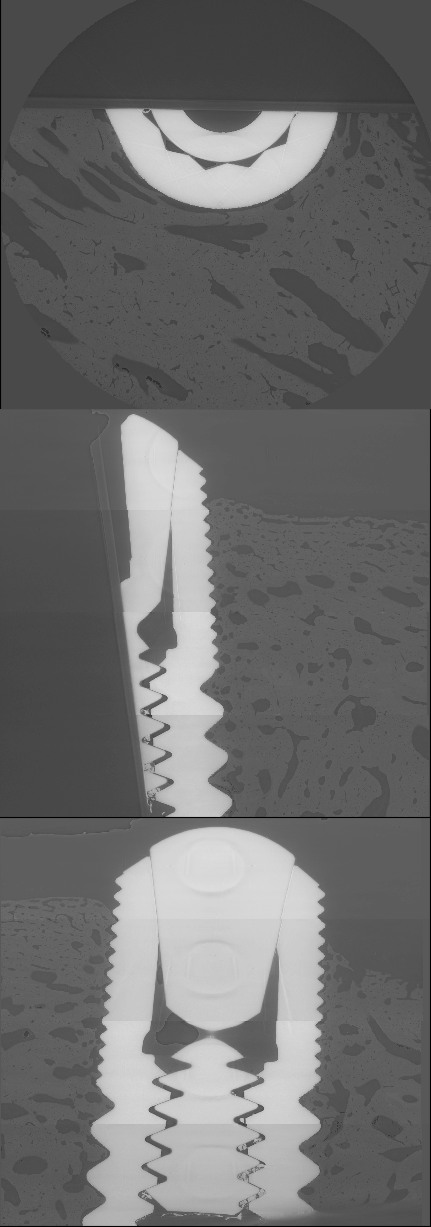
\includegraphics[scale=0.50]{figures/3_view_sample.png}
\caption{\aleksandar{Temporary example figure of sample in x,y,z dimension. It could perhaps even be manually annotated (meaning we can indicate roughly what regions correspond to: resin, air, implant, bone), and related to the physical scale mentioned above? Maybe as simple as overlaying a ruler with the given scale?}}
\label{fig:3viewsample}
\end{figure}

Each material has a different density and thus absorption. The titanium implant has higher absorption than bone.
Bone material then has higher absorption than its sorrounding tissue, vessels, air and resin.

\subsubsection*{Data acquisition}

It can be difficult to study and evaluate the bone structure and blood network without destroying or
manipulating the sample. X-ray computed tomography is a widely used tool for non-intrusive medical
imaging. By exposing a subject to X-rays, we can map the linear attentuation coffecient of the passing
rays. Each ray is attenuated relatively to the density and composition of the material it passes. By
rotating either the scanner or the sample we can get a full 3D image representation of the inner
structure of the sample. Each volumetric pixel (voxel) then represents the X-ray attenuation at its spatial position. We can therefore reliably use X-rays to internally characterise samples in a non-intrusive and non-destructive manner. Regular CT-scans can provide spatial resolutions on the order of millimetre scale.\aleksandar{ref} The more modern micro computed tomography ($\mu$CT) can provide much higher spatial resolution on the micrometre scale.\aleksandar{ref} Both setups utilize poly-energetic beams, which can cause artifacts around high density regions. This effect is called beam-hardening\aleksandar{ref}, and occurs when rays with lower energy are attenuated more frequently. This offsets the local contrast, by overestimating the attenuation, leaving lighter spots on the image. Many other types of artifacts will also occur in these common scanners, but most is taken into account by calibration using phantoms and pre-hardening the beam before it reaches the sample. Due to its common usage, much software also exists to correct for noise and smaller imperfections during reconstruction\aleksandar{ref}.

This work focuses on data acquired by Synchrotron Radiation micro-CT (SR$\mu$CT). For this imaging
technique, electrons are accelerated to ultra-relativistic speeds in trajectories directed by strong
magnetic fields. Contrary to both CT and $\mu$CT, this approach requires a large particle accelerator, and is not standard medical or laboratory equipment\aleksandar{ref}. The added complexity means that SR$\mu$CT can offer an even better spatial resolution of up to 0.1 $\mu$m. The resulting beams are high in brilliance and collimation which gives a very clear signal. Its mono-energetic nature also means that images are not subject to artifacts from beam-hardening.

\aleksandar{Can we confirm whether data was acquired at the ESRF and at which beamline? Also which energies were used? All this could be important for reproducibility.}

\aleksandar{Was filtered backprojection used to do reconstruction, and who has done that? Was it done at ESRF?}

\subsubsection*{Image data}

A single image sample contains voxels with of spatial resolution 1.875$\mu$m. The physical size of
a sample is about 6.5mm, which makes the raw dimensions of a single image $(3480,3480,3384)$ pixels.
For computational purposes, this has been cropped to be divisible by $2^5=32$. A full image sample
is further split into 4-6 sub-volumes through the height of the implant. This gives a size of $(3456,3456,810)$ pixels per sub-volume, where the last axis gets stacked for a full volume.

\aleksandar{OBS: 846 i rå størelse, 810 er efter volume-matching.}

\aleksandar{Important to explain a bit about how the samples were cut during acquisition. How were the samples secured in order not to be shifted too much etc.}

\section*{Physical effects, noise and artifacts}

Noise in tomography is unavoidable, and it makes segmentation harder. Matarials may be well separated from certain angles in the 3d-reconstructed image, but overlap from others. Some noise like that corrected by flat-field correction is very uniformly distributed across images. Some noise is however very spatially dependent on its sorrounding regions. Since we know the compositions of the materials being imaged, we can counter some of these effects during segmentation. The noise effects manifest themselves as numerical shifts in voxel-values as a function of their position. This is a direct result of a misrepresented attenuation along the axis the X-rays are passing. 

\aleksandar{perhaps we should mention at what energies the data is taken. This helps to narrow which types of effects play into the data.}

Low energy rays contribute mostly with noise from scattering effects. A ray will propagate through a material, get scattered and diffract from its initial trajectory. This gives a misrepresentation of the attenuation along its initial trajectory.

Streaking artifacts from dense implant region, but also in the transition from bone to softer tissue.

...

For SR$\mu$CT a high photon flux allows for very short exposure times \citep{srexptime}.
This can help counter noise from suboptimal counting statistics\citep{srnoise}.


* Gå fra brede effekter som viser sig i hele billedet (og er mere generelle) -> Til de mere specifikke effekter som er mere specifikke for vores case

* genskær fra voxels
mørke effekter modsat lysere effekter fra beam-hardening (x-rays er inverteret)

Forklare hvorfor vi ser mørke områder, særligt at det mørke lægger sig omkring implantatet,
men at det så aftager mod knoglen, for så at blive kraftigere og bredere helt ved knoglen..
nok refraktion osv. \aleksandar{OBS: before talking about specific noise in our data, we should probably include one or more examples of noise that shows how the segmentation is made harder due to this noise.}


\section*{Solutions}

\aleksandar{Work-in-progress}

Individual materials are segmented from the full image, which is represented by their respective histograms.

\begin{equation}
H(x,v) = \sum_{m=1}^{n} g_{m}(x,v) + r(x,v)
\end{equation}

Where $g_m$ represents a histogram for materials $m\in\{1,n\}$, and $r(x,v)$ is incorrectly identified remainding region.

We find the probability for a certain material as:

\begin{equation}
p(m|x,v) = \frac{g_{m}(x,v)}{H(x,v)}
\end{equation}

We then have a single distribution is given by a piecewise polynomial:

\begin{equation}
g_{m}(x,v) = a_{m}(x) e^{ -b_{m}(x) |v-c_{m}(x)|^{d_{m}(x)} }
\end{equation}

Where a is the height, b is the width, c is the centre and d is the exponent.

If we were to look at the distributions for individual slices, we would get too much variance.
Instead we would like to fit the individual coefficients to get a smooth function.

\subsection*{Miscellaneous}

We shall go through these subjects and explain what was done and how + why. We briefly explain how the method works.

\begin{itemize}
 \item Volume matching
 \item Find implant mask
 \item EDT (Euclidean distance transform)
 \item Gauss
 \item Gauss + EDT
 \item Hist(x,y,z,r)
 \item Find lines / ridges
 \item Get distributions
 \item Beskrive processen under GUI trinvist
 \item Segment materials from distributions
 \item Bayesian combination of materials from their distributions
\end{itemize}

\subsection*{Probabilities}

\aleksandar{Work-in-progress}

Ud fra et 3d-billede (volumen), kan vi tælle os til de enkelte fordelinger

p(I), p(I|x), p(I|y), p(I|z), p(I|r), hvor $r=\sqrt{(x-x_0)^2+(y-y_0)^2}$

ved at finde peaks og fitte distributioner kan vi da finde approksimationer til

p(c|I), p(c|I,x), p(c|I,y), p(c|I,z), p(c|I,r)

hvor c er klasserne, fx knogle, blodåre, væv, ... 

Vi vil gerne finde kombinationsfordelinger som kan klassificere voxels ved brug af mere information end kun intensiteten - blandt andet hvor voxelen befinder sig.

Ud fra fx p(c|I,x) og p(c|I,y) og ... vil vi gerne approksimere p(c|I,x,y,z,r) uden at skulle repræsentere den eksplicit som et kæmpe volumen.

Dette vil vi gøre ved at bruge betinget uafhængiged. \aleksandar{Evt inkludere bevis for at det er validt. Ellers så blot forklare hvordan sandsynlighederne sammensættes og bruges.}


\section{Method}\label{sec:method}
% Spatial correlation 2d histograms (den nemme, 1 2d hist)
In this section, we will describe the method for exploiting spatial correlation based on the
2D-histograms of the tomographies. We will start by motivating the problem, then give an overview
of how we solve the problem, with a final detailed walkthrough of each step in the overall workflow.

\subsection{1-dimensional histograms}
%diskuter overlappende materialer
Looking at a 1D-histogram of the voxel value in a tomography, as shown in~\Cref{fig:1d-hist}, we are
able to distinguish different distributions, but we see that there is a large overlap. This leads to
global thresholding being infeasible, at least for the distributions in the lower half of the histogram.
This happens because the voxel value is not globally defined, as~\Cref{sec:physics} explains, which
illustrates how the different materials cover ranges of values that blend together in the histogram.

\begin{figure}
    \centering
    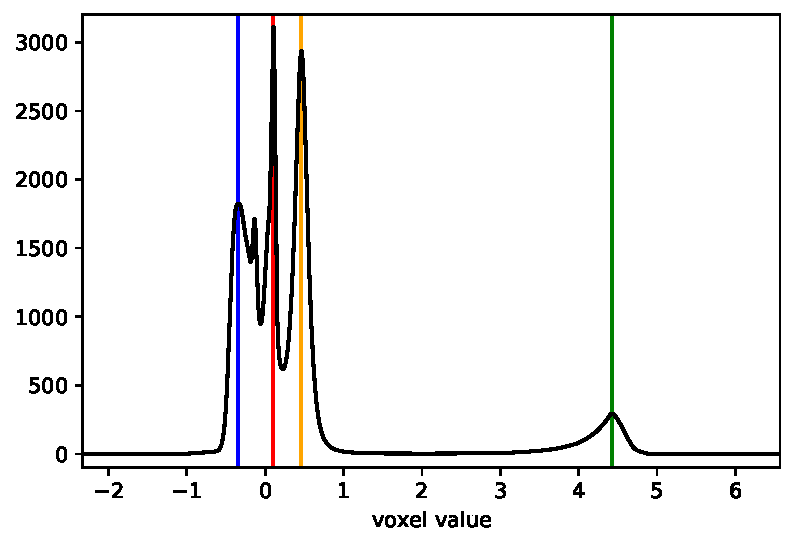
\includegraphics[width=\linewidth]{1d_hist.pdf}
    \caption{1-dimensional histogram of the voxel values of a tomography. The blue line is air peak,
    the red line is the soft tissue peak, the green line is the bone peak, and the orange line is
    the implant peak.}
    \label{fig:1d-hist}
\end{figure}

\subsection{Preprocessing}\label{sec:preprocess}
To reduce the complexity of the segmentation process, we preprocess the data by removing redundant
information. From our work in an upcoming paper under preparation, we are able to obtain two
masks: an \textit{implant mask} and a \textit{bone mask}.

Since the values of the implant material is radically different from the rest of the sample, obtaining
the rough implant mask through global thresholding is trivial, as the orange line in~\Cref{fig:1d-hist}
shows. This mask is then refined, along with the internal gaps being closed, giving us the implant mask.
Using this mask, we are also able to remove the air making up half of the sample cylinder. This is depicted
in~\Cref{fig:3viewsample}, above the implant and to the left of the implant in the XY and YZ cross
sections respectively. Finally the implant mask can show us the orientation of the implant. This squashes
the blue peak from the histogram, leaving the two peaks marked by the red and green lines as being
the most defined.

As we are only interested in the voxels inside the bone, and we know that bone is the most prominent
material left, we perform another coarse segmentation. This is done by thresholding between the two
large distributions, choosing everything to the right of this threshold as the bone mask. These voxels
are morphologically closed, to also consumes the internal gaps in the bone region, which makes up the
soft tissue inside the bone. The implant and bone region masks are applied throughout subsequent steps
to filter out noise in the tomography.

\subsection{Exploiting spatial information}
% Show the correlation of x,y,z,r to histograms 2d
As described in~\Cref{sec:physics}, the voxel values vary according to their positioning, motivating
us to utilize spatial information in the tomography. In order to include spatial information,
we consider \textit{expanding} a dimension to produce multiple 1D histograms into a combined 2-dimensional
histogram. Each 2D histogram is computed by locking the dimension in question and produce the 1D histograms.
Specifically, we consider the radius ($r$) dimension from the center of the implant, as the voxel values
vary most, closest to the implant. The algorithm for computing the 2-dimensional histogram for the
radius can be seen in~\Cref{alg:2dhists} with the resulting 2D histogram plotted in~\Cref{fig:2dhists}.
From this plot, we see two prominent distributions that change along the $r$ axis. This is however
not an accurate representation, as the edges of the implant are not uniformly spread across the longest
axis of the implant. This means that the radius does not sufficiently represent the distance from the
implant at high resolutions. This is shown in~\Cref{fig:edt-vs-diffusion}, where we see that a radius
of constant value from the center has varying distance to the implant.

% Kept for historical reasons.
%\begin{algorithm}
%    \caption{2-dimensional histograms. Allocation also implies zero initialization.}
%    \label{alg:2dhists}
%    \begin{algorithmic}
%        \Function {2D\_hist} {$voxels[n_z,n_y,n_x],c_x,c_y,n_{bins},v_{min},v_{max}$}
%            \State $n_r \gets \left\lfloor\sqrt{\left\lfloor \frac{n_x}{2} \right\rfloor^2 + \left\lfloor \frac{n_y}{2} \right\rfloor^2}\right\rfloor+1$
%            \State \textbf{allocate} $h_z[n_z,n_{bins}], h_y[n_y,n_{bins}]$
%            \State \textbf{allocate} $h_x[n_x,n_{bins}], h_r[n_r,n_{bins}]$
%            \For {$z,y,x$ \textbf{in} $0{:}n_z,0{:}n_y,0{:}n_x$}
%                \State $v \gets voxels[z,y,x]$
%                \If {$v_{min} \leq v \leq v_{max}$}
%                    \State $v_{i} \gets (n_{bins}-1) \cdot \frac{v - v_{min}}{v_{max} - v_{min}}$
%                    \State $r \gets \left\lfloor\sqrt{(x-c_x)^2 + (y-c_y)^2}\right\rfloor$
%                    \State $h_z[z,v_{i}]{+}{+}$
%                    \State $h_y[y,v_{i}]{+}{+}$
%                    \State $h_x[x,v_{i}]{+}{+}$
%                    \State $h_r[r,v_{i}]{+}{+}$
%                \EndIf
%            \EndFor
%            \Return $h_z,h_y,h_z,h_r$
%        \EndFunction
%    \end{algorithmic}
%\end{algorithm}

\begin{algorithm}
    \caption{2-dimensional radius histogram.}
    \label{alg:2dhists}
    \begin{algorithmic}
        \Function {hist\_r} {$voxels[n_z,n_y,n_x],c_x,c_y,n_{bins},v_{min},v_{max}$}
            \For {$z,y,x$ \textbf{in} $0{:}n_z,0{:}n_y,0{:}n_x$}
                \State $v \gets voxels[z,y,x]$
                \If {$v_{min} \leq v \leq v_{max}$}
                    \State $v_{i} \gets (n_{bins}-1) \cdot \frac{v - v_{min}}{v_{max} - v_{min}}$
                    \State $r \gets \left\lfloor\sqrt{(x-c_x)^2 + (y-c_y)^2}\right\rfloor$
                    \State $h_r[r,v_{i}]{+}{+}$
                \EndIf
            \EndFor
            \Return $h_r$
        \EndFunction
    \end{algorithmic}
\end{algorithm}

\begin{figure}
    \centering
    %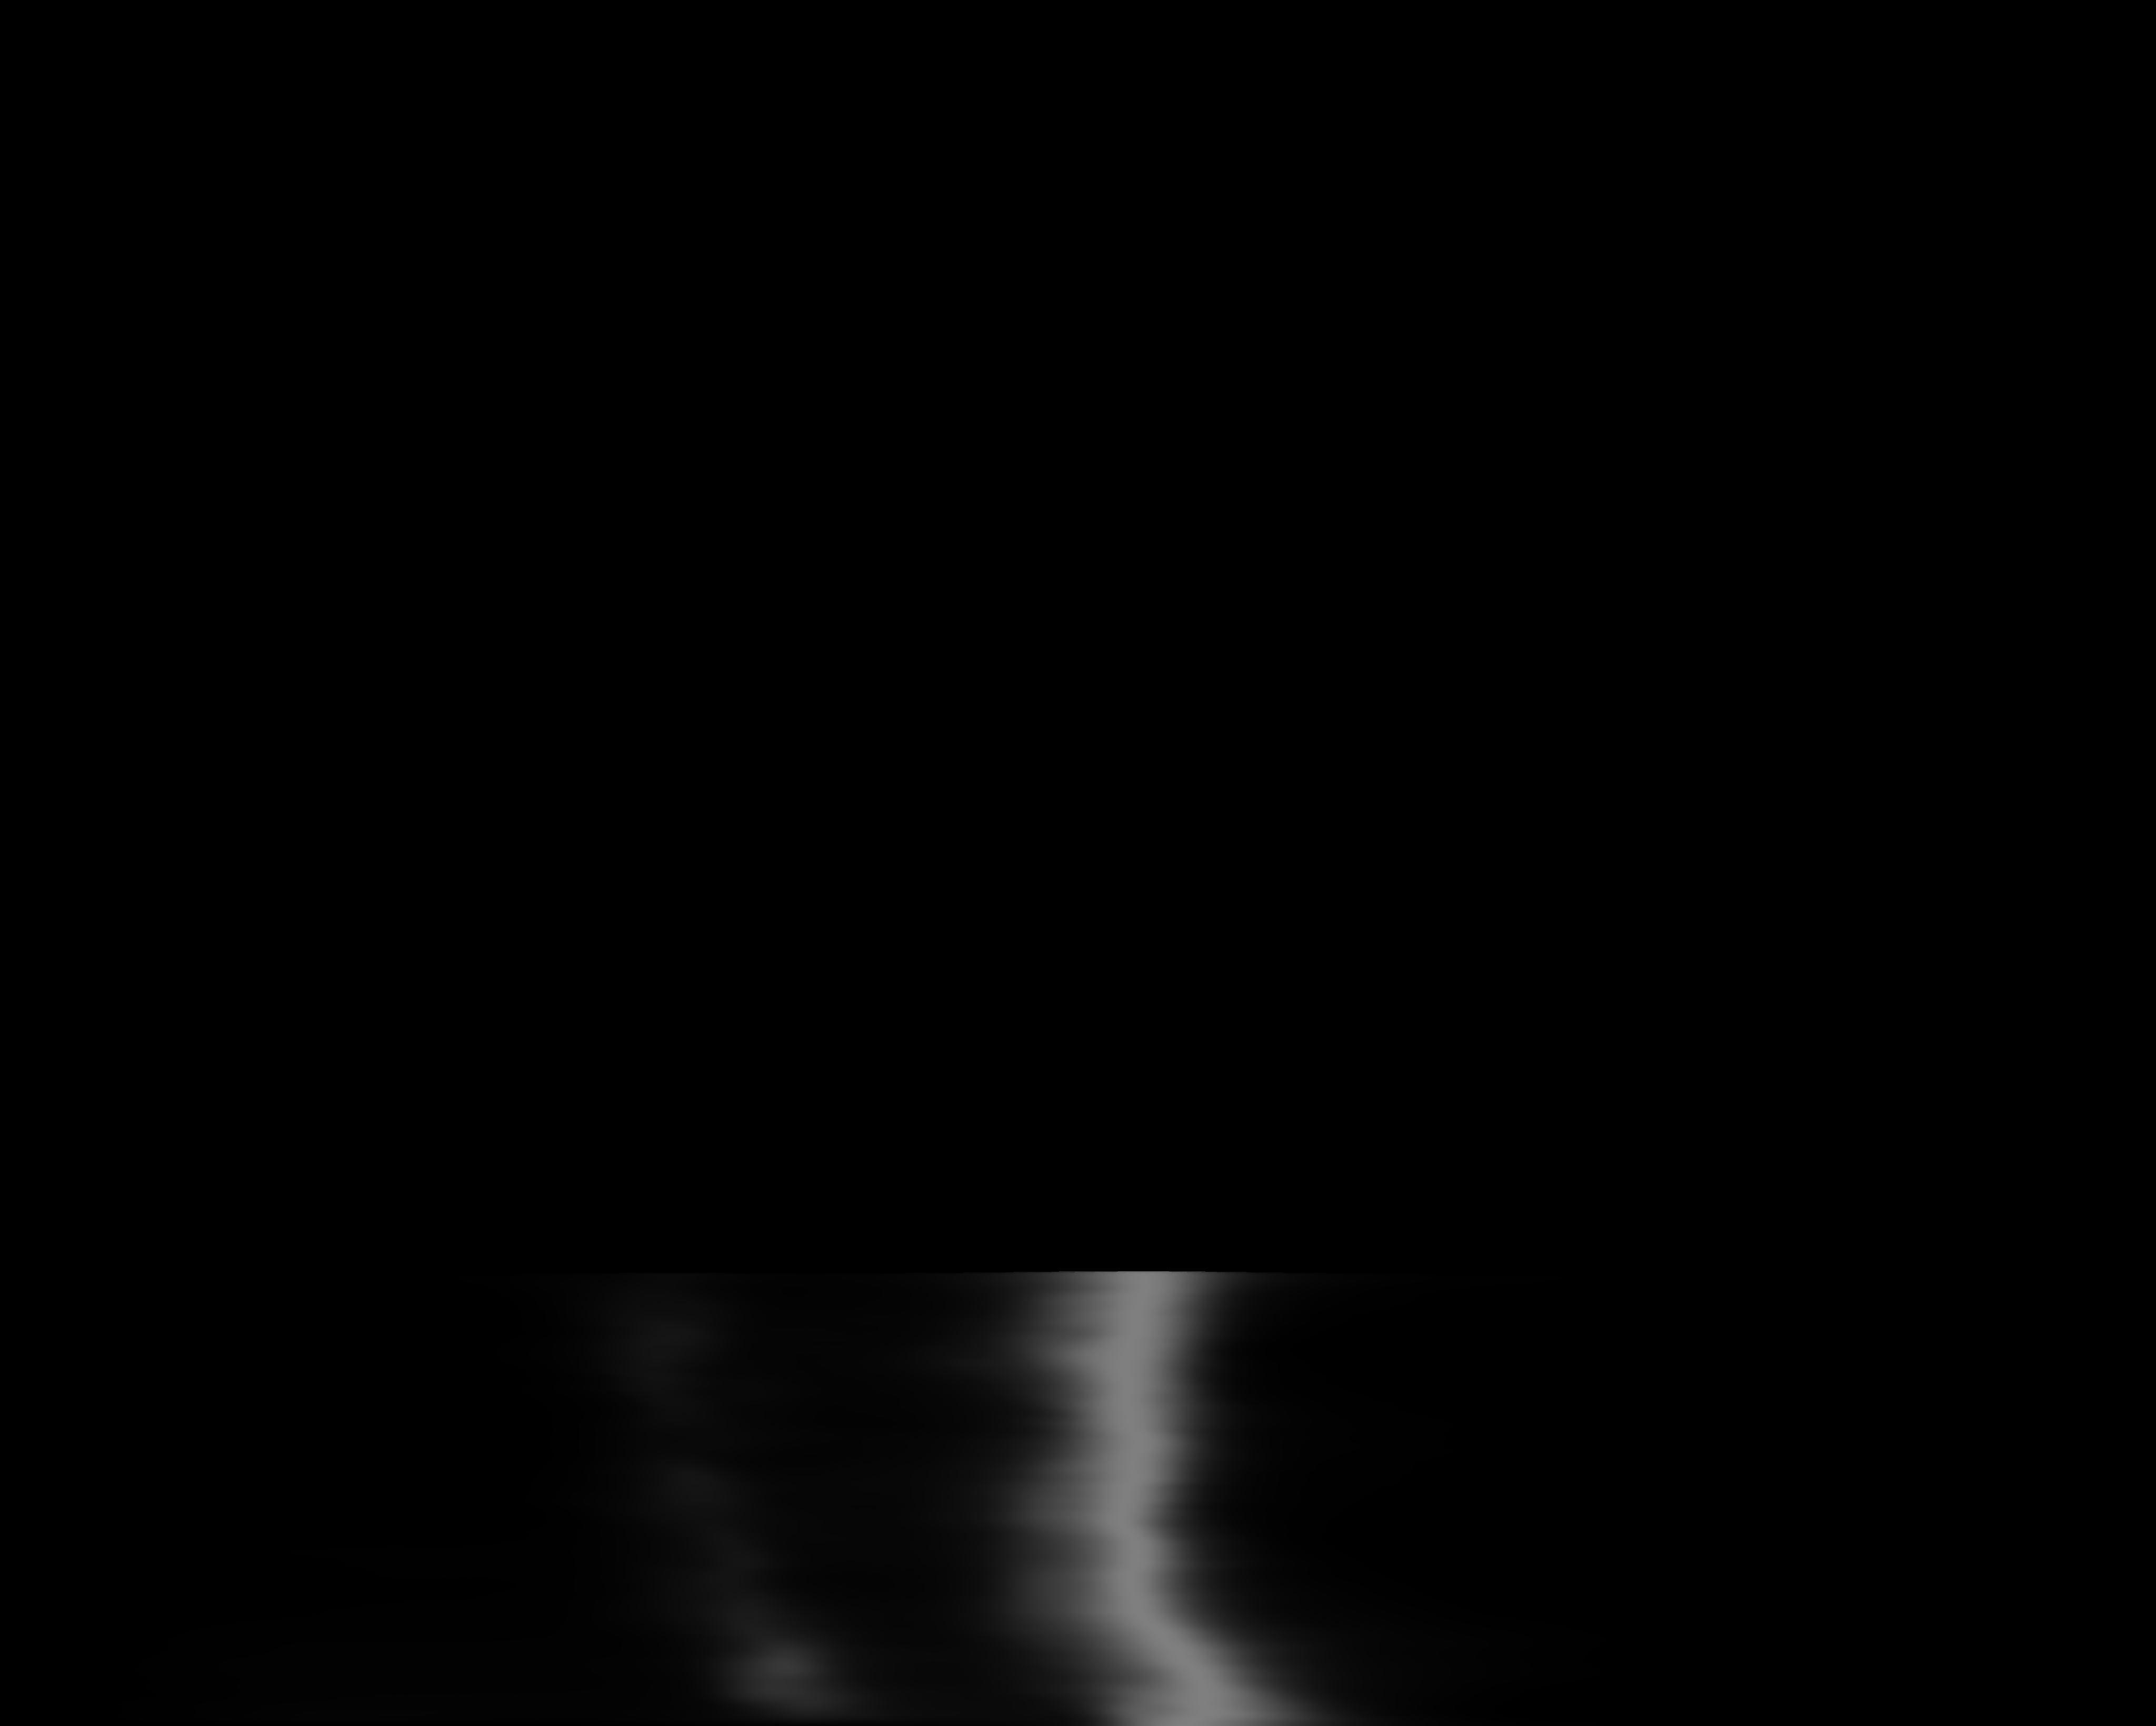
\includegraphics[width=.49\linewidth]{zb-bone_region3.png}
    %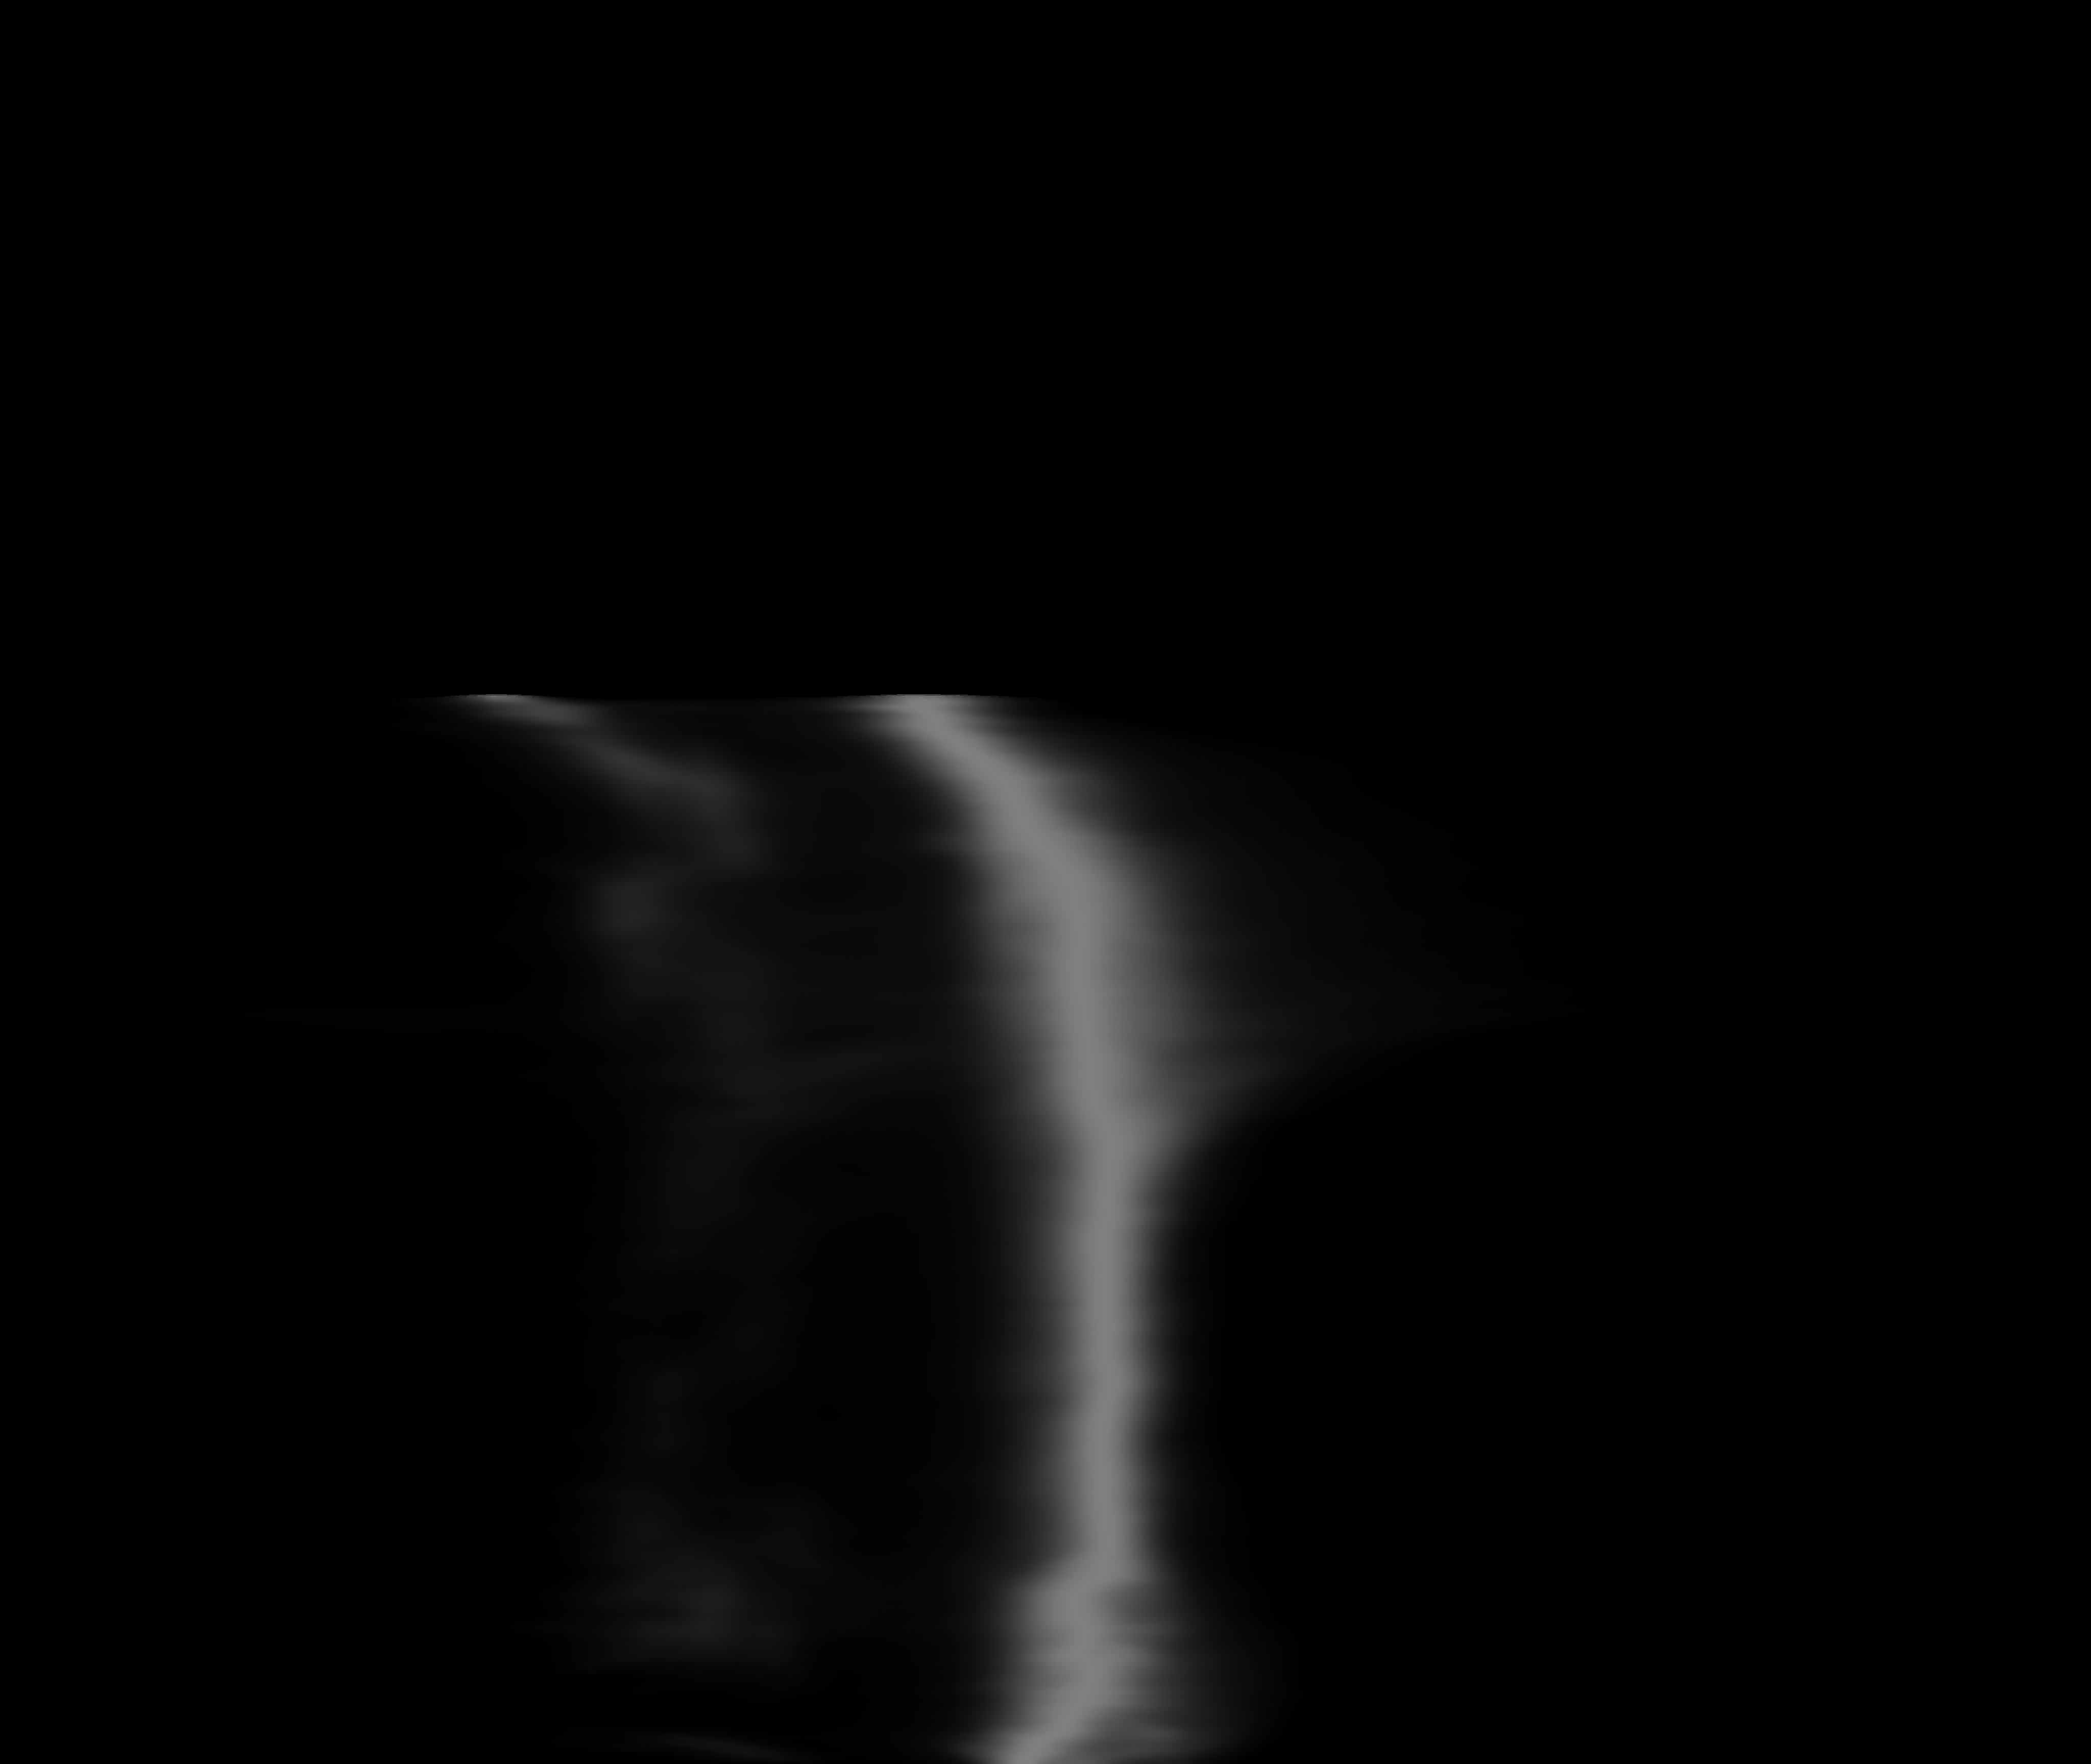
\includegraphics[width=.49\linewidth]{yb-bone_region3.png}
    %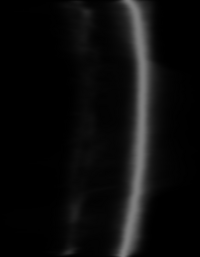
\includegraphics[width=.49\linewidth]{xb-bone_region3.png}
    %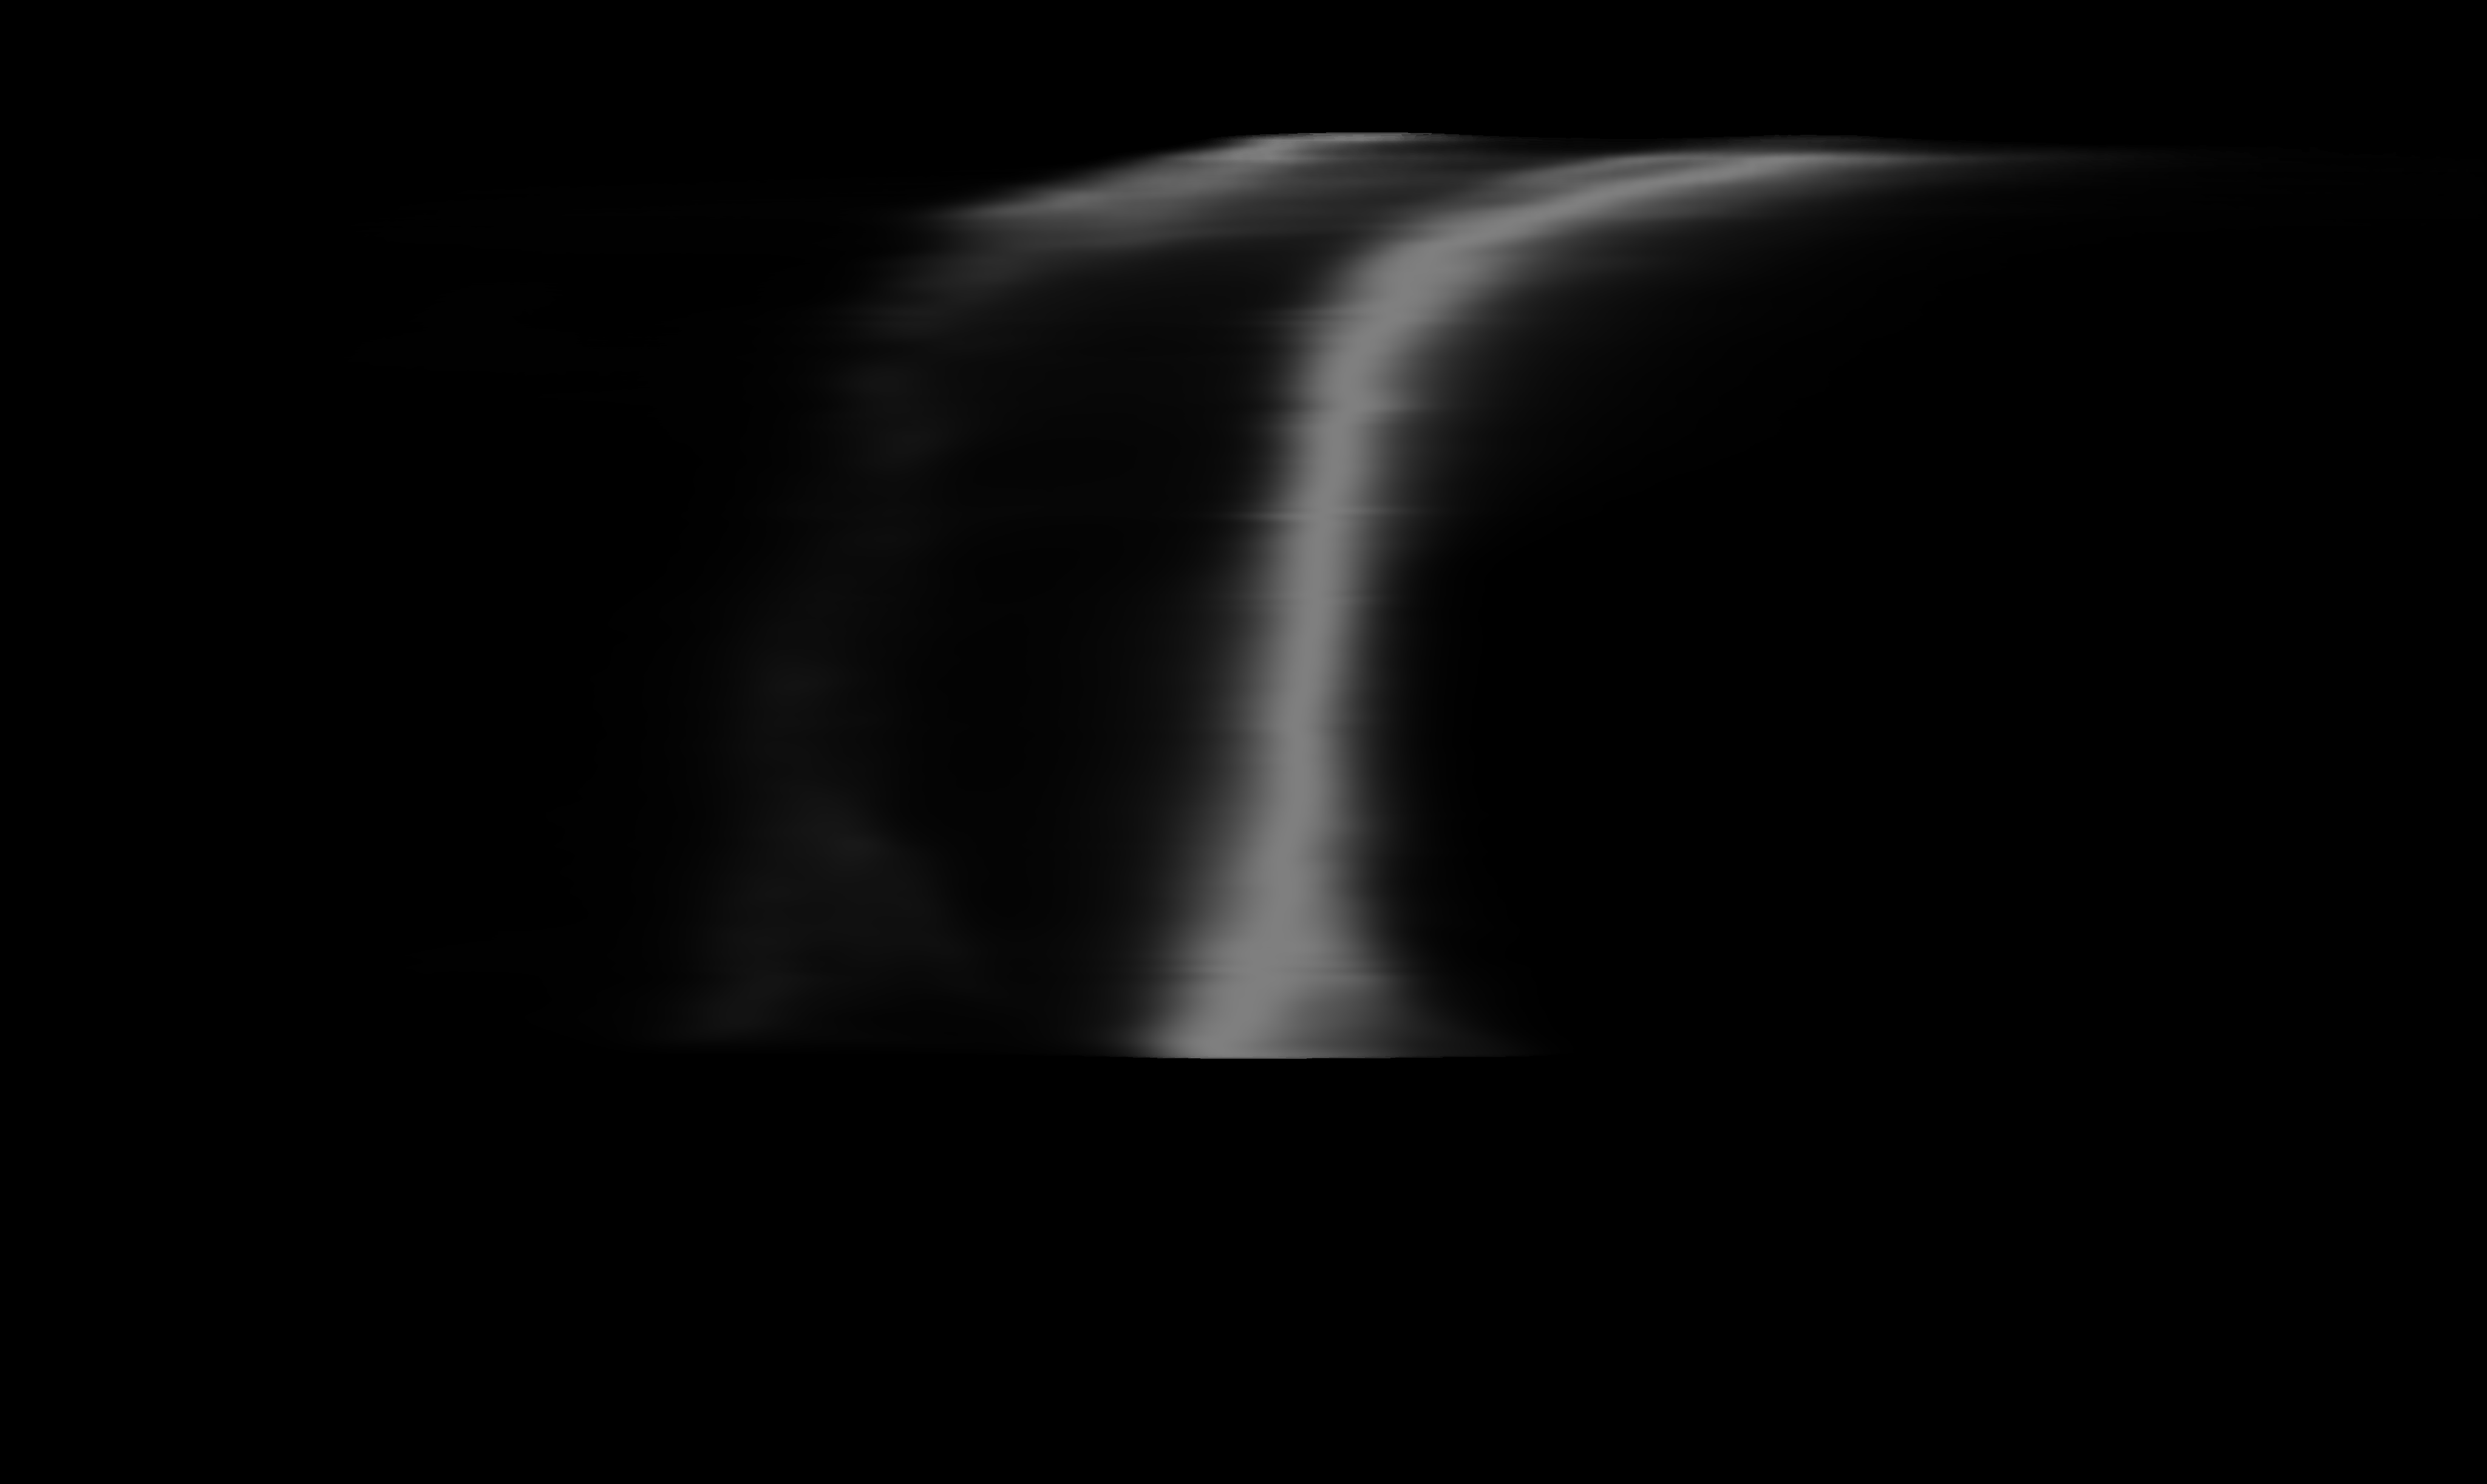
\includegraphics[width=\linewidth]{rb-bone_region3.png}
    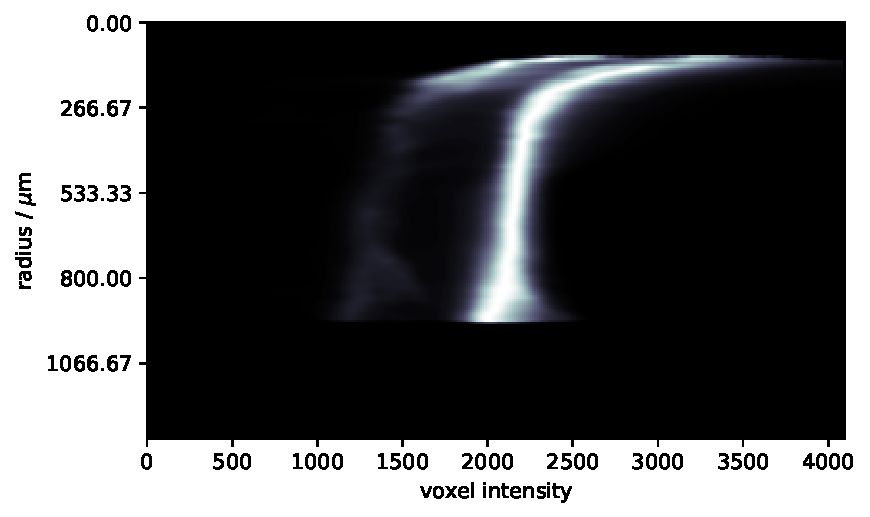
\includegraphics[width=\linewidth]{rb-bone_region3.pdf}
    \caption{2D radius histogram. The y-axis depicts radius, with the x-axis being voxel value.}
    \label{fig:2dhists}
\end{figure}

\subsection{Field histograms}
%Show that the fields can perfectly seperate
%discuss all the way to implant contact
In order to obtain spatial information based on the relation to the implant, we construct two
\textit{field} representations: Euclidian Distance Transform (EDT) and Diffusion.

%EDT is good overall, but difficult close to the implant.
EDT computes each voxel as the Euclidian distance to the implant.  This makes for a generally good
representation for all but the voxels that are close to the implant. The shortcoming near the implant
is mainly due to the fact that the voxels in the grooves of the implant have the same distance, and
thus the same value, as voxels next to the threads of the implant. This is shown in~\Cref{fig:edt-vs-diffusion}.
As discussed in~\Cref{sec:beam-hardening}, the implant produces a \textit{glowin}g effect, which
should be corrected by having higher field values for voxels surrounded by implant.

%Use diffusion to "zoom in" on the implant, as it is good close to the implant, but throws everything far away into the same bin
To get better correction close to the implant, we utilize diffusion where the implant "glows" further
accumulating the value when a voxel is surrounded by implant. This is shown in~\Cref{fig:edt-vs-diffusion},
where the voxels in the grooves are affected by multiple implant voxels. A slice of the resulting
diffusion field can be seen in~\Cref{fig:field-slice}.

\begin{figure}
    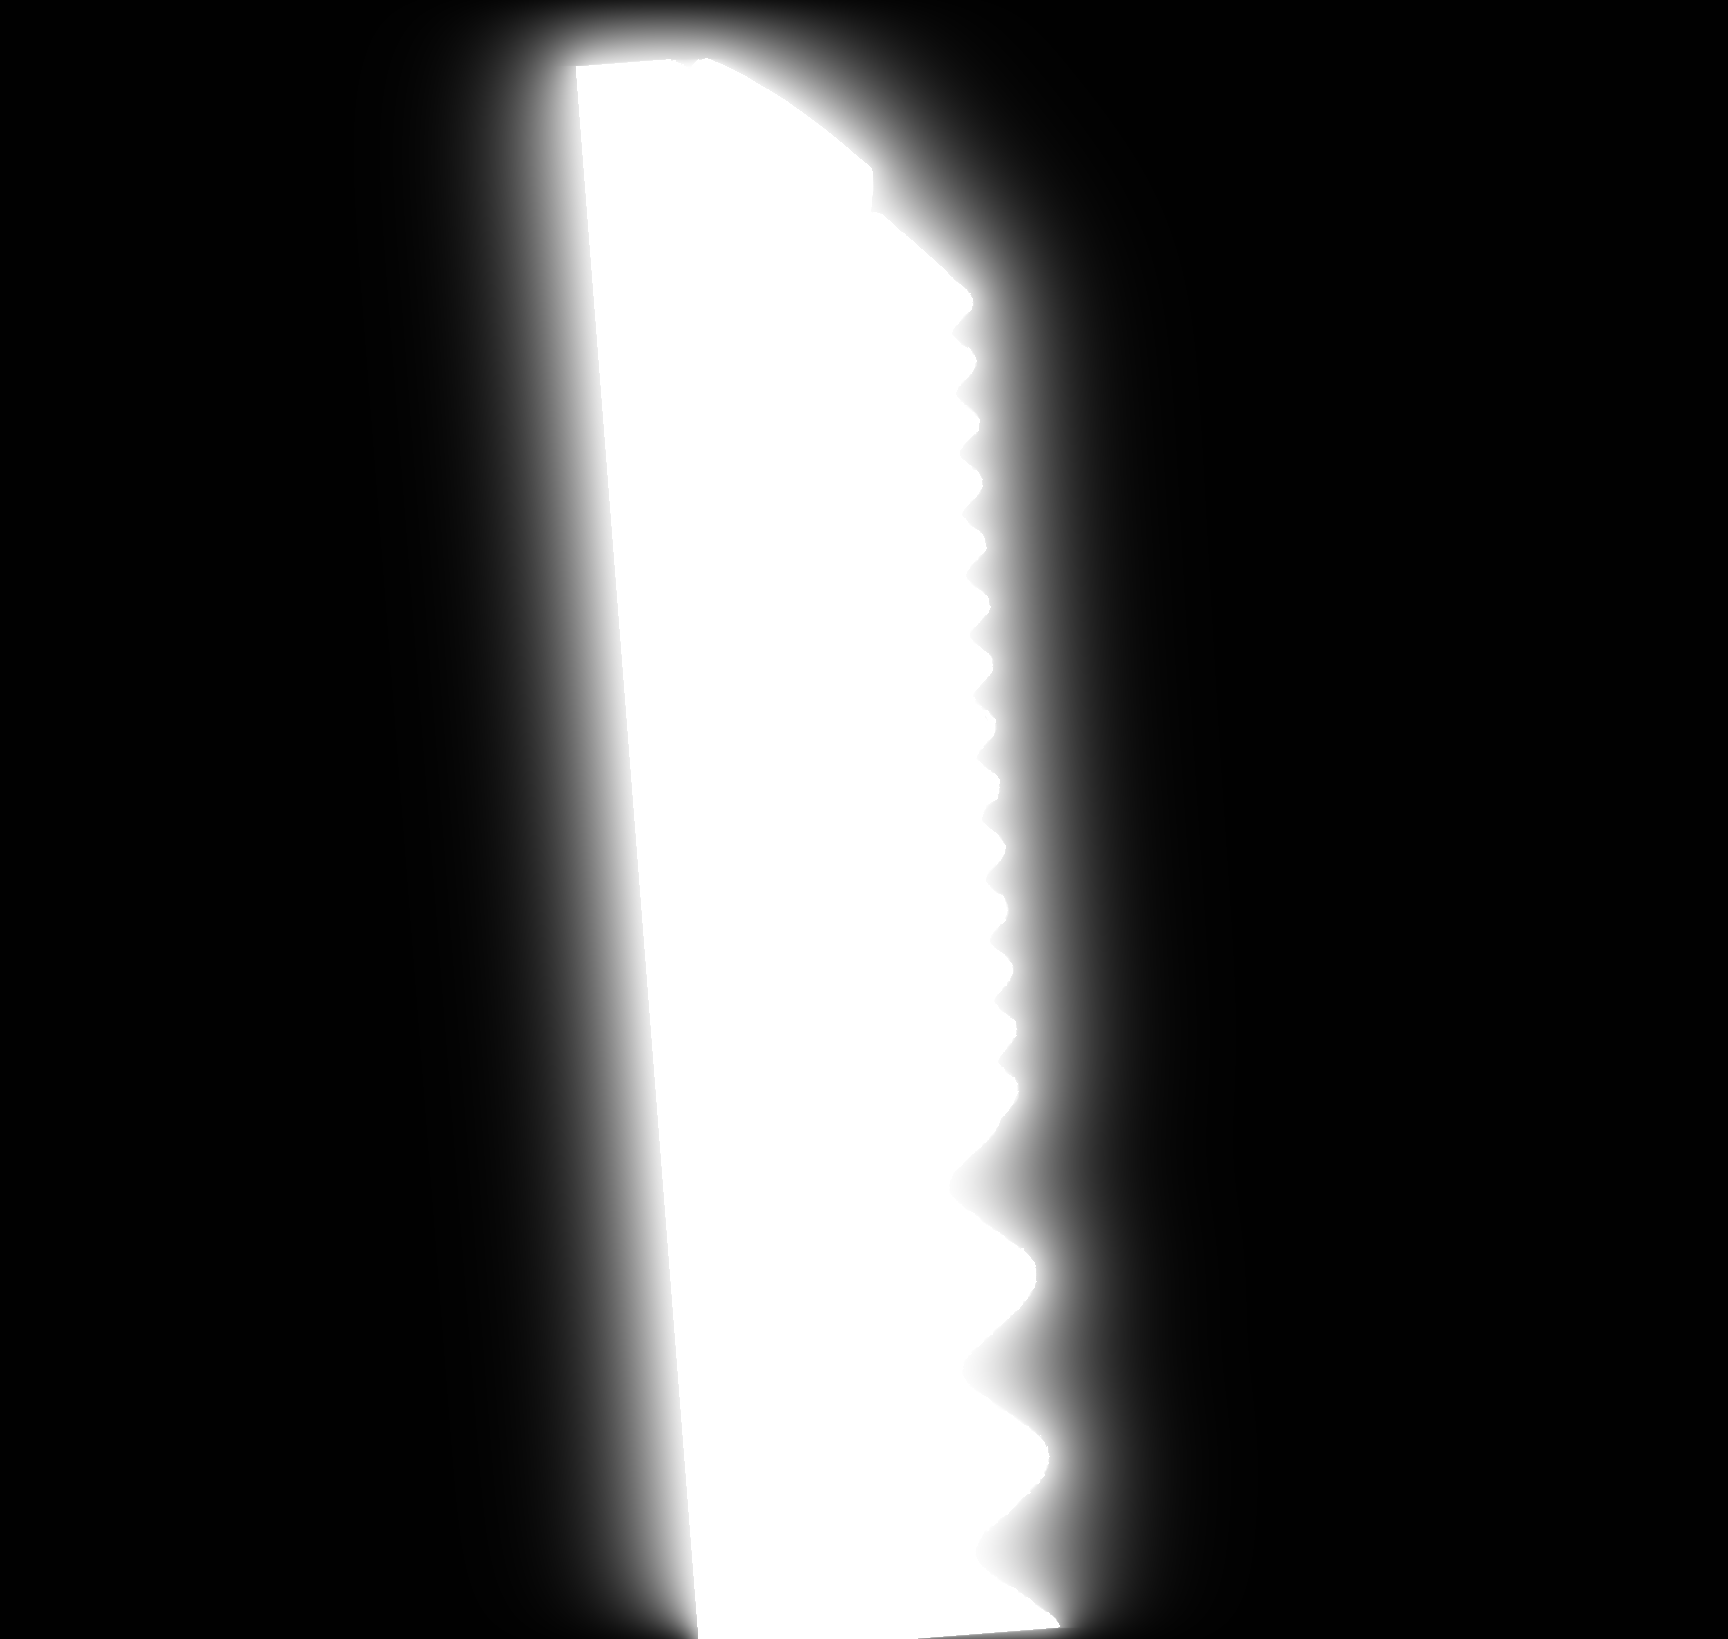
\includegraphics[width=\linewidth]{770c_pag-gauss-yz.png}
    \caption{A slice of the diffusion field in the YZ plane.}
    \label{fig:field-slice}
\end{figure}

\begin{figure}
    \vspace{-1.5cm}
    \centering
    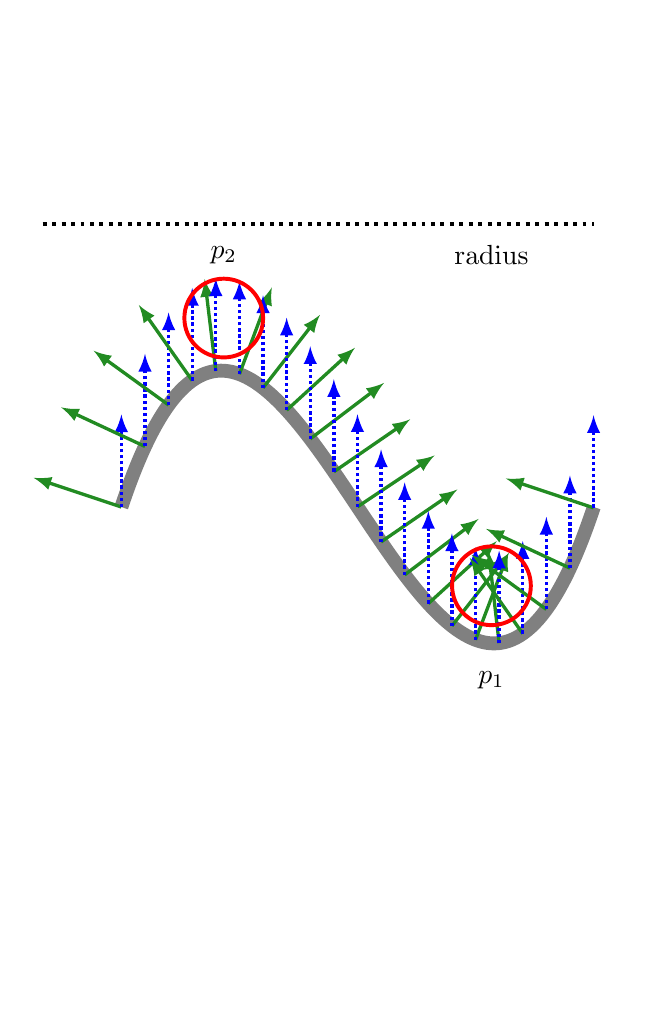
\begin{tikzpicture}[scale=2.0]
        \draw[gray,line width=5pt] (0,0)
        .. controls (1,3) and (2,-3) .. (3,0)
        \foreach \p in {0,5,...,100} {
          node[sloped,inner sep=0cm,above,pos=\p*0.01,
          anchor=south,
          minimum height=1.0cm,minimum width=1.0cm]
          (N \p){}
        }
        \foreach \p in {0,5,...,100} {
          node[midway,above,inner sep=0cm,above,pos=\p*0.01,
          anchor=south,
          minimum height=1.0cm,minimum width=1.0cm]
          (N2 \p){}
        }
        ;
        \foreach \p in {0,5,...,100} {
          \draw[-latex,ForestGreen, very thick] (N \p.south) -- (N \p.north);
          \draw[-latex,blue,densely dotted, very thick] (N2 \p.south) -- (N2 \p.north);
        }
        \draw[red, line width=0.5mm] (0.65,1.20) circle (0.25cm);
        \node at (0.65,1.60) {$p_2$};
        \draw[red, line width=0.5mm] (2.35,-0.5) circle (0.25cm);
        \node at (2.35,-1.10) {$p_1$};
        \draw[black, line width=0.5mm, dotted] (-0.5,1.8) -- (3.0,1.8);
        \node at (2.35,1.60) {radius};
      \end{tikzpicture}
      \vspace{-3.5cm}
    \caption{Visualization of the different field computations close to the implant threading in the YZ plane. The EDT is depicted in blue, where we see that $p_1$ and $p_2$ have the same distance. Diffusion is depicted in green, where we see multiple arrows contributing to the value of $p_1$. Using a radius of constant value, we see that the distance to the implant varies a lot.}
    \label{fig:edt-vs-diffusion}
\end{figure}

While diffusion works well on voxels close to the implant, it assigns the same value to the voxels
far from the implant. Therefore, an optimal solution is to use both the EDT and the diffusion field
to better represent both voxels that are far away, as well as the ones that are close to the implant.
We achieve this by adding the two fields together, producing a final combined field.

% Show that the distance to the implant in edt will be the same in the grooves of the screw compared
% to the threads of the screw. This is "fixed" with diffusion, as the grooves will be brigher as it
% is surrounded by more implant.

\subsection{Walkthrough of the method}
This section will describe each step of our method in detail. Going from tomography to a segmented tomography.

\subsubsection{Overview}
%Coarse steps, explain the idea
In order to reach the tissue-bone implant contact metric, we have the three coarse steps: compute the fields, segmentation using the fields, and extraction of the contact from the segmented tomography.

The steps of the field computation are:
\begin{itemize}
    \item Compute the EDT and Diffusion fields to give each voxel spatial information about its relation to the implant.
    \item Compute frequency distributions of voxel values as functions of field values as 2D histograms.
\end{itemize}

Then, in order to segment using the fields:
\begin{itemize}
    \item Find the materials within the 2D histograms as ridges, using image processing techniques.
    \item From the ridges, compute initial approximate frequency distributions of each material, which are then optimized to fit the 2D histograms.
    \item From the optimized distributions, we derive probability distributions for material classification. These distributions approximate the conditional probabilities $P(m|v,x)$ that a particular voxel belongs to material $m$ given that it has voxel value $v$ and field value $x$.
    \item Apply the probability distributions to the tomography, segmenting the voxels into the different materials.
\end{itemize}

Finally, to produce the tissue-bone implant contact metric:
\begin{itemize}
    \item From the segmented tomography, we compute the blood network of the bone regions to further extract which soft tissue voxels that are blood vessels.
    \item This blood network is used alongside the the segmented bone to produce the final metric.
\end{itemize}

%\james{TODO: Forklar bedre. Adskil ny segmenteringsmetode og anvendelse til BIC}

These steps are also summarized in the flow chart in~\Cref{fig:flowchart}.

\begin{figure}
    \centering
    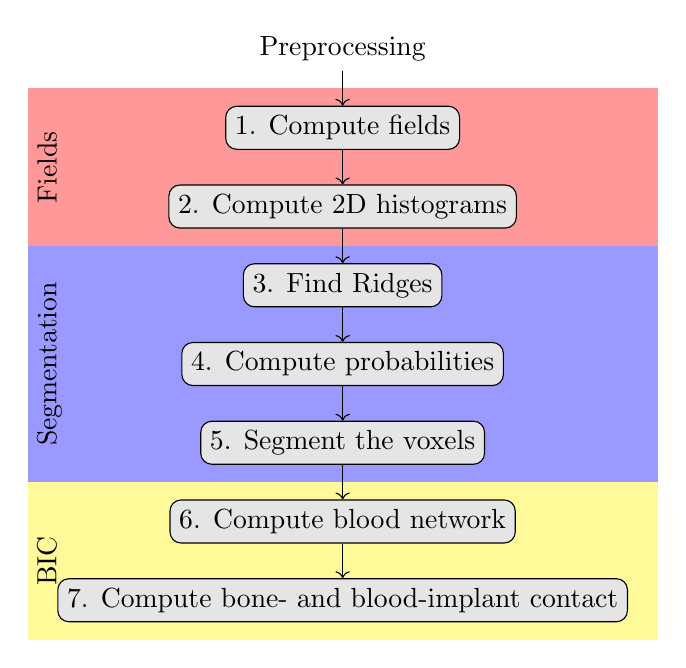
\begin{tikzpicture}
        \fill[red!40] (-4,.5) rectangle (4,-1.5);
        \fill[blue!40] (-4,-1.5) rectangle (4,-4.5);
        \fill[yellow!40] (-4,-4.5) rectangle (4,-6.5);
        \node[rotate=90, anchor=north] (field) at (-4,-.5) {Fields};
        \node[rotate=90, anchor=north] (segment) at (-4,-3) {Segmentation};
        \node[rotate=90, anchor=north] (bicc) at (-4,-5.5) {BIC};

        \node       (prep)  at (0, 1) {Preprocessing};
        \node[draw, fill=black!10, rounded corners] (field) at (0, 0) {1. Compute fields};
        \node[draw, fill=black!10, rounded corners] (hists) at (0,-1) {2. Compute 2D histograms};
        \node[draw, fill=black!10, rounded corners] (curvs) at (0,-2) {3. Find Ridges};
        \node[draw, fill=black!10, rounded corners] (probs) at (0,-3) {4. Compute probabilities};
        \node[draw, fill=black!10, rounded corners] (segm)  at (0,-4) {5. Segment the voxels};
        \node[draw, fill=black!10, rounded corners] (blood) at (0,-5) {6. Compute blood network};
        \node[draw, fill=black!10, rounded corners] (bic)   at (0,-6) {7. Compute bone- and blood-implant contact};

        \path[draw, ->] (prep)  -- (field);
        \path[draw, ->] (field) -- (hists);
        \path[draw, ->] (hists) -- (curvs);
        \path[draw, ->] (curvs) -- (probs);
        \path[draw, ->] (probs) -- (segm);
        \path[draw, ->] (segm)  -- (blood);
        \path[draw, ->] (blood) -- (bic);
    \end{tikzpicture}
    \caption{Flowchart depicting the steps of the method.}
    \label{fig:flowchart}
\end{figure}

\subsubsection{Segmentation}
The overall segmentation is computed in steps 1-5. For each step we will describe the process, showing
the algorithm where applicable, along with the the intermediate results.

\vspace{\baselineskip}
\noindent\textit{\textbf{Step 1: Field computations}}
Both fields are computed from the implant mask, as described in~\Cref{sec:preprocess}.
EDT is computed using the Python package \texttt{edt}~\cite{pypi-edt}. It takes the implant mask and
sets every non-set voxel to be the Euclidian distance of the nearest implant voxel.

For diffusion, rather than solving the diffusion equation, we approximate it using multiple convolutions
of a 3D-Gaussian kernel. Furthermore, instead of a single pass with a 3D-kernel, we apply 3 $\times$ 1D
convolutions, one in each dimension, to the tomography. This obtains the same result as a regular 3D-Gaussian
kernel. The algorithm can be seen in~\Cref{alg:diffusion}, and the XZ-plane in~\Cref{fig:field-slice}.

\begin{algorithm}
    \caption{Diffusion approximation.}
    \label{alg:diffusion}
    \begin{algorithmic}
        \Function {Diffusion} {$voxels[n_z*n_y*n_x]$, $repitions$, \newline \indent \indent $kernel[2*k+1]$}
            \State $S \gets [n_y * n_x, n_x, 1]$
            \State $N \gets [n_z, n_y, n_x]$
            \State $buf_0[:] \gets voxels[:]$
            \For {$rep$ \textbf{in} $repitions$}
                \For {$dim$ \textbf{in} $dimensions$}
                    \For {$z,y,x$ \textbf{in} $0{:}n_z,0{:}n_y,0{:}n_x$}
                        \State $X \gets [z,y,x]$
                        \State $i_{start} \gets - \min (k, X[dim])$
                        \State $i_{end} \gets \min (k, N[dim] - X[dim] - 1)$
                        \State $i_{global} \gets z*S[0] + y*S[1] + x*S[2]$
                        \For {$i$ \textbf{in} $i_{start}:i_{end}$}
                            \State $i_{offset} \gets i_{global} + i*S[dim]$
                            \State $buf_1[index] \gets buf_0[i_{offset}] * kernel[i+k]$
                        \EndFor
                    \EndFor
                    \State $buf_0[:] \gets buf_1[:]$
                \EndFor
            \EndFor
            \Return $buf_0$
        \EndFunction
    \end{algorithmic}
\end{algorithm}

%EDT + Diffusion
To obtain a good seperation both close to the implant and far away, we combine the two fields into a
single one as shown in~\Cref{eq:field-comb}.

%\begin{algorithm}
%    \caption{Field combination}
%    \label{alg:field-comb}
%    \begin{algorithmic}
%        \Function {field\_combine} {$f_{edt}, f_{dif}$}
%            \State $r \gets f_{dif} - \frac{f_{edt}}{\max (f_{edt})}$
%            \State $r \gets r - \min (f_{dif})$
%            \State $r \gets \frac{r}{\max (f_{dif})}$
%
%            \Return $r$
%        \EndFunction
%    \end{algorithmic}
%\end{algorithm}

\begin{equation}
    \label{eq:field-comb}
    \begin{split}
        f_{combined} &= \frac{f_{diffusion} - \frac{f_{edt}}{\max (f_{edt})} \min (f_{diffusion})}{\max (f_{diffusion})}
    \end{split}
\end{equation}

\vspace{\baselineskip}
\noindent\textbf{Step 2: 2D histograms} \\

From the combined fields we compute a 2D-histogram with the field value on the y-axis and the voxel
value on the x-axis.  This allows us to see the distribution of voxel values, based on their
relative position from the implant. The algorithm for the field-histogram can be seen in~\Cref{alg:field-hist}
along with a plot of the resulting histogram in~\Cref{fig:field-hist}. We see that the voxel values
shift based on their closeness to the implant, which clearly results in two seperable distributions.

\begin{algorithm}
    \caption{Field 2D histograms.}
    \label{alg:field-hist}
    \begin{algorithmic}
        \Function {Field\_hist} {$voxels[n_z,n_y,n_x]$, $field[n_z,n_y,n_x]$, $v_{bins}$, \indent \indent $v_{min}$, $v_{max}$, $f_{bins}$, $f_{min}$, $f_{max}$}
            \For {$z,y,x$ \textbf{in} $0{:}n_z,0{:}n_y,0{:}n_x$}
                \State $v \gets voxels[z,y,x]$
                \If {$v_{min} \leq v \leq v_{max}$}
                    \State $f \gets voxels[z,y,x]$
                    \If {$f_{min} \leq f \leq f_{max}$}
                        \State $v_i \gets (v_{bins} - 1) - \frac{v - v_{min}}{v_{max} - v_{min}}$
                        \State $f_i \gets (f_{bins} - 1) - \frac{f - f_{min}}{f_{max} - f_{min}}$
                        \State $h[f_i,v_i]{+}{+}$
                    \EndIf
                \EndIf
            \EndFor
            \Return $h$
        \EndFunction
    \end{algorithmic}
\end{algorithm}

\begin{figure}
    %
\includegraphics[width=\linewidth]{fb-edt-bone_region3.png}
    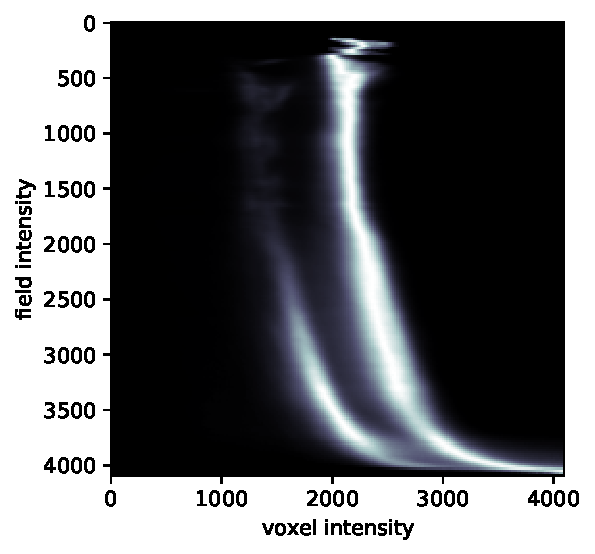
\includegraphics[width=\linewidth]{fb-gauss+edt-bone_region3.pdf}
    \caption{2D field histogram. Note that there are two clearly seperated ridges, which makes up
    different materials.}
    \label{fig:field-hist}
\end{figure}

\vspace{\baselineskip}
\noindent\textbf{Step 3: Isolate the materials} \\
The next step is to isolate the different materials spatially, which is done through the field-histogram.
For our first attempt, we applied Otsu's threshold to each each row in the 2D-histogram. While this
provided good results for two well defined distributions, it eventually began to fail. This was either
because of lack of samples, or because the histogram did not contain two distributions, which is an
underlying assumption of Otsu thresholding. These two effects occurred at the edges (both closest and
furthest from implant), which would bleed into the later steps of the segmentation process.

Rather than finding the threshold value in between the distributions, our next solution was to start
finding the distributions by finding the ridges of the 2D-histogram. We do this by applying a series
of image processing techniques, described in~\Cref{alg:material}. Each of the resulting contours
become their own material, which are then labeled as material 1 or 2 respectively for this particular
sample. For samples that would contain more than two distributions, the same algorithm should apply,
as long as the distributions does not overlap.

\begin{algorithm}
    \caption{Material isolation.}
    \label{alg:material}
    \begin{algorithmic}
        \Function {Materials} {$h[f_{bins}$, $v_{bins}]$, $\sigma$, $peak_{min}$, $k_x$, $k_y$, \newline \indent \indent $i_{dilate}$,$i_{erode}$, $t$}
            \For {$row$ \textbf{in} $0{:}f_{bins}$}
                \State $r \gets gaussian\_smooth(h[row,:], \sigma)$
                \State $p \gets find\_peaks(r, peak_{min})$
                \State $ps[p] \gets 1$
            \EndFor
            \State $kernel = cross\_kernel(k_x, k_y)$
            \State $d \gets dilate(ps, i_{dilate}, kernel)$
            \State $e \gets erode(d, i_{erode}, kernel)$
            \State $cs \gets find\_contours(e)$
            \For {$i$ \textbf{in} $0{:}|cs|$}
                \If {$size(cs[i]) > t$}
                    \State $l \gets draw\_contour(l, cs[i], i+1)$
                \EndIf
            \EndFor
            \Return $l$
        \EndFunction
    \end{algorithmic}
\end{algorithm}

\begin{figure*}
    % %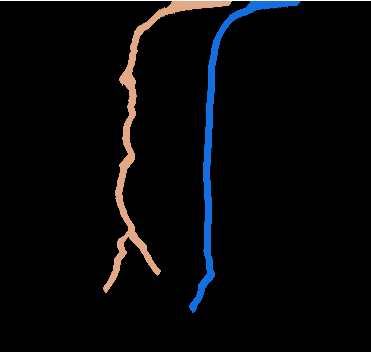
\includegraphics[width=0.5\linewidth]{curves_edt.png}%
    % %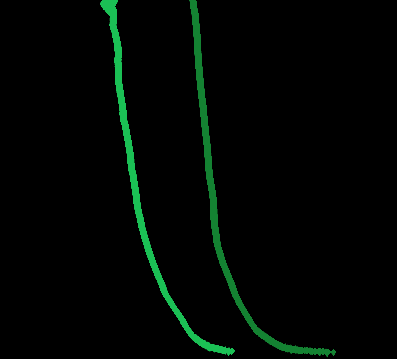
\includegraphics[width=0.5\linewidth]{curves_diffusion.png}
    % 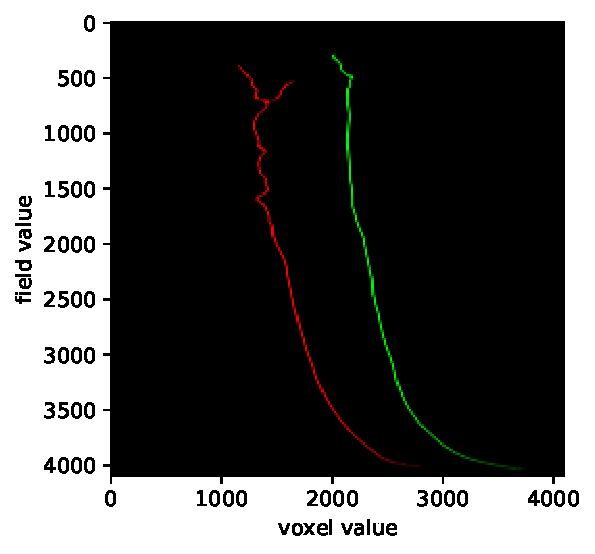
\includegraphics[width=\linewidth]{ridges_gauss+edt-bone_region3.pdf}
    % \james{will produce overall plot with probabilities}
    % \caption{Detected ridges from the combined field histogram.}
    % \label{fig:curves}
  \centering
  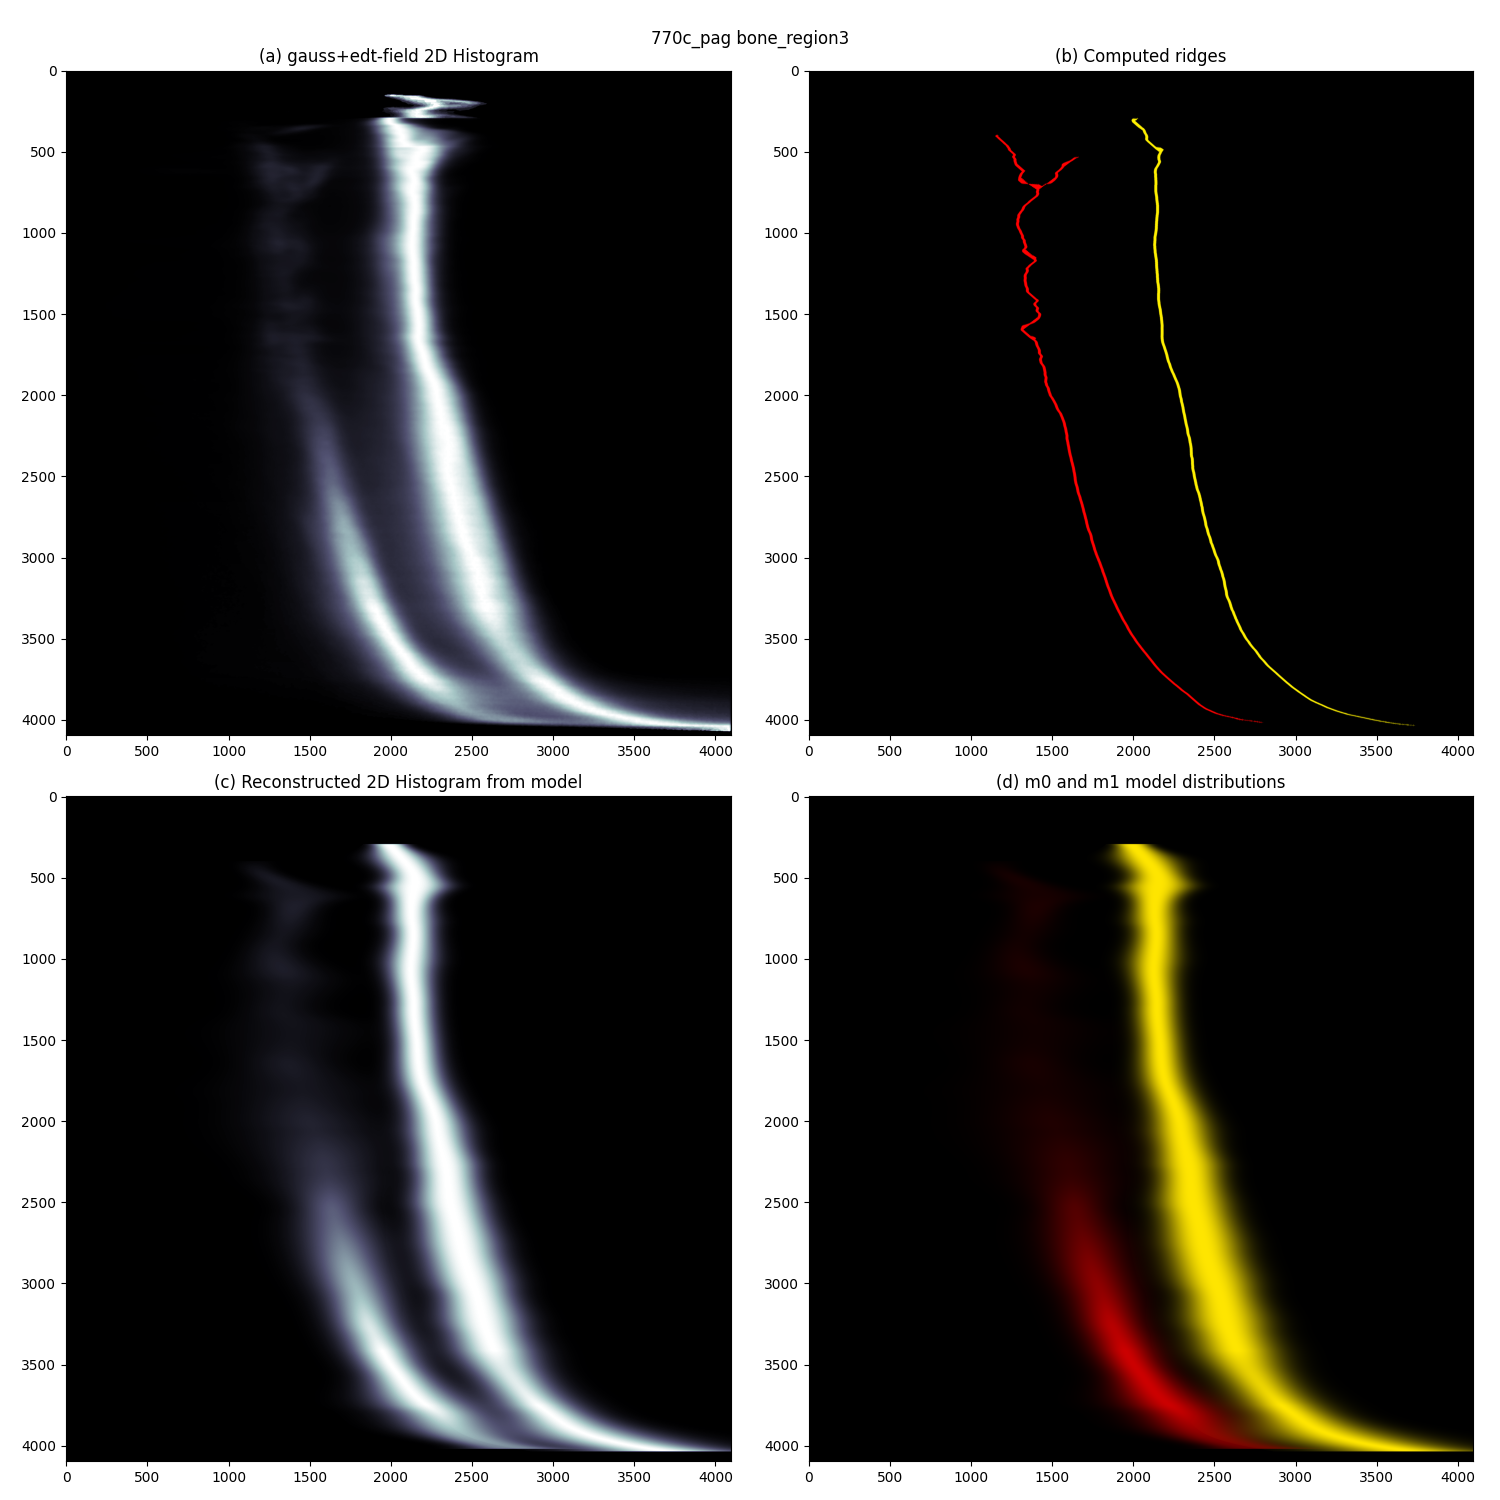
\includegraphics[width=.9\textwidth]{compute_probabilities_gauss+edt_bone_region3}\\
  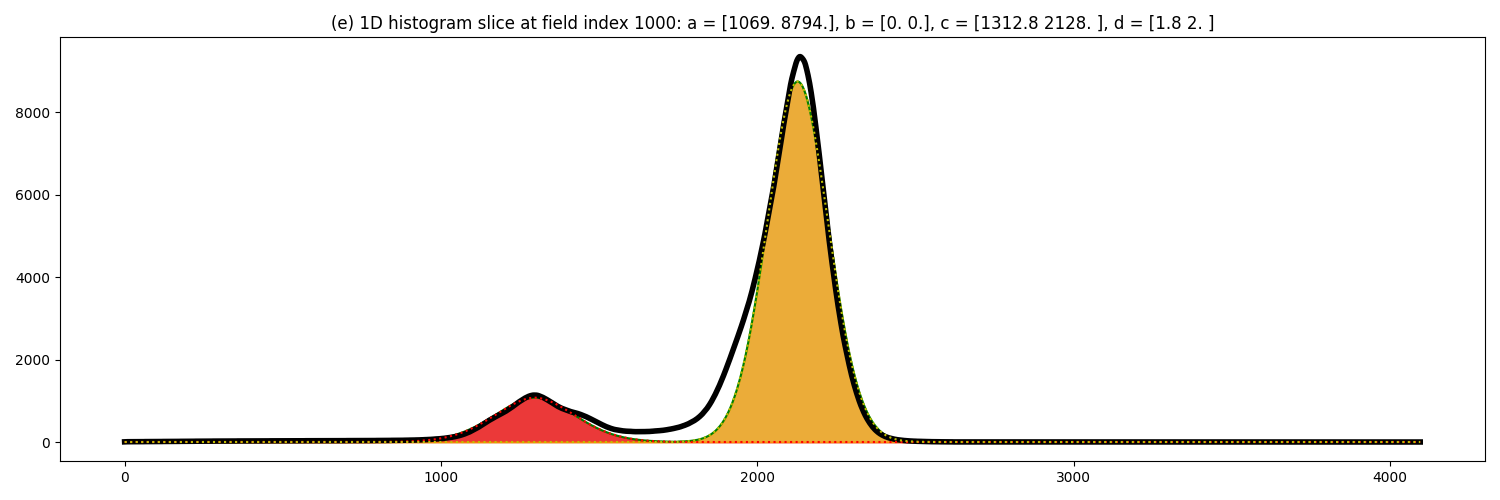
\includegraphics[width=.9\textwidth]{hist_slice_gauss+edt_bone_region3}\\
  \caption{(a) Measured 2D histogram for the compund diffusion+distance field from Step 2. (b)
    The detected ridges from Step 3. (c) Sum of computed frequency distribution models
    with optimized smooth piecewise cubic functions for parameters $a(\fval), b(\fval), c(\fval), d(\fval)$:
    this is the part of the 2D histogram explained by the smooth model. (d) The individual distributions evaluated
    on the 2D field-value$\times$ voxel-value grid. (e) A single 1D slice of the 2D histogram (black) together with
    the model frequency distributions. Red is soft-tissue, yellow is bone mineral.
  }
  \label{fig:curves-and-more}
\end{figure*}

\vspace{\baselineskip}
\noindent\textbf{Step 4: Compute models for material probability distributions} \\
Our goal is to obtain good conditional probability distributions $P(m|v,\xx)$
that model the likelihood of a voxel having material type $m$ as a function
both on its value $v$ and its position $\xx$ in space. For the probabilities
conditioned on the field values (distance or diffusion field), we model
the probability distributions $P(m|v,f(\xx))$ conditioned on
voxel- and field values. We want to make sure that these distribution
functions vary smoothly across space (or as a function of field values),
to ensure that we can identify the materials correctly across the entire
image: i.e., even though the frequency distributions look completely different
close to the titanium implant compared to the middle region or sample surface,
we can track the unbroken, smooth deformation to assign a global material
identity.

To this end, we first {\it model the frequency distributions} using the
2D histograms. Given that we are modeling materials $m=1,\ldots,M$,
we write the full 2D histogram as a sum of distributions
$g_m(\fval,v)$ modeling the described part, and an undescribed
residual $r(\xx,v)$.
\begin{equation}
  \label{eq:hist}
  H(\fval,v) = \sum_{m=1}^M g_m(\fval,v) + r(\fval,v)
\end{equation}
The residual is constrained to be non-negative, i.e., we must not explain
more voxels than the image contains.
The distribution functions can be chosen in any way that approximately
model the observed frequencies: we first used Gaussians with passable success,
but found that they dropped off too rapidly. We instead found excellent results
with the next-simplest model, leaving the exponential power free:
\begin{equation}
  \label{eq:dist-form}
  g_m(\fval,v) = a_m(\fval) e^{-b_m(\fval) |v-c_m(\fval)|^d_m(\fval)}
\end{equation}
where for each field value $\fval$
$a(\fval)$ is the distribution height at the center $v=c(\fval)$,
$b(\fval)$ is the exponential falloff rate, and $d(\fval)$ is
the exponential power ($d=2$ yields a Gaussian, $d=1$ a simple exponential).
In practice we found $1.5\le d \le 2$ to best match the actual frequency
distribution decay rates.

Using the ridges found in the previous step, we generate good starting
guesses and constraints for the distribution parameters
$a,b,c,d$:
For each field-value $\fval$ (corresponding to a row in the 2D histogram),
we initialize the starting approximation as:
\begin{equation}
  \label{eq:starting-guesses}
  \begin{split}
    c_m(\fval) &= \mathop{\mathtt{argmax}}_{v \text{ with }\lab[\fval,v] = m} H(\fval,v)    \\
    a_m(\fval) &= H(\fval,c_m(\fval))\\
    b_m(\fval) &= 3/\mathrm{width}_m(\fval)^2 \\
    d_m(\fval) &= 2
  \end{split}
\end{equation}
where we use half the distance to the center of ridge $m+1$ as the width
$\mathrm{width_m}(\fval)$, using the relation that $b = 3/w^d$ yields
a $5\%$ cutoff at $w$ when $1\le d \le 2$. This approximation
already yields a good approximation. Thus, the subsequent
optimization using the constrained quasi-Newton optimization method L-BFGS-B\cite{BFGS}
converges rapidly to an excellent fit. Each 1D histogram row is first optimized
independently in parallel: The resulting numerical functions
$a_m(\fval),\ldots,d_m(\fval)$ are then converted into piecewise cubic
functions using a least squares-based algorithm that ensures continuity
and differentiability across the piecewise segments. This lets us interpolate across
outliers due to noise, but equally important:
extrapolate our models smoothly into the regions very close to the implant, where
we don't have enough voxels to produce good statistics.

We finally obtain the {\it conditional probabilities} from the material frequency distribution
models $g_m$ as:
\begin{equation}
  \label{eq:Pm}
  P(m|v,f(\xx)) = \frac{g_m(v,f(\xx))}{H(v,f(\xx))}
\end{equation}
(well-defined where $H(v,\fval) > 0$, zero outside this region as $0\le g_m \le H$).



%%% Local Variables:
%%% mode: latex
%%% TeX-master: "main"
%%% End:


\vspace{\baselineskip}
\noindent\textbf{Step 5: Perform segmentation}

The final step of the segmentation process is to utilize the probabilities for segmentation.
This process is fairly straightforward, as each voxel is looked up in the probability distribution,
which carries the same shape as the field-histogram.

\begin{algorithm}
    \caption{Final segmentation from the probability distributions.}
    \label{alg:segment}
    \begin{algorithmic}
        \Function {Segment} {$voxels[n_z,n_y,n_x], p[f_{bins},v_{bins}],$ \newline \indent \indent $v_{bins}, v_{min}, v_{max}, f_{bins}, f_{min}, f_{max}$}
            \For {$z,y,x$ \textbf{in} $0{:}n_z,0{:}n_y,0{:}n_x$}
                \State $v \gets voxels[z,y,x]$
                \If {$v_{min} \leq v \leq v_{max}$}
                    \State $f \gets voxels[z,y,x]$
                    \If {$f_{min} \leq f \leq f_{max}$}
                        \State $v_i \gets (v_{bins} - 1) - \frac{v - v_{min}}{v_{max} - v_{min}}$
                        \State $f_i \gets (f_{bins} - 1) - \frac{f - f_{min}}{f_{max} - f_{min}}$
                        \State $result[z,y,x] \gets p[f_i, v_i]$
                    \EndIf
                \EndIf
            \EndFor
            \Return $result$
        \EndFunction
    \end{algorithmic}
\end{algorithm}

\subsection{Results of the field-segmentation}

Here we present the final output from the steps described above.

\begin{figure}
    \centering
    \begin{subfigure}[b]{\linewidth}
        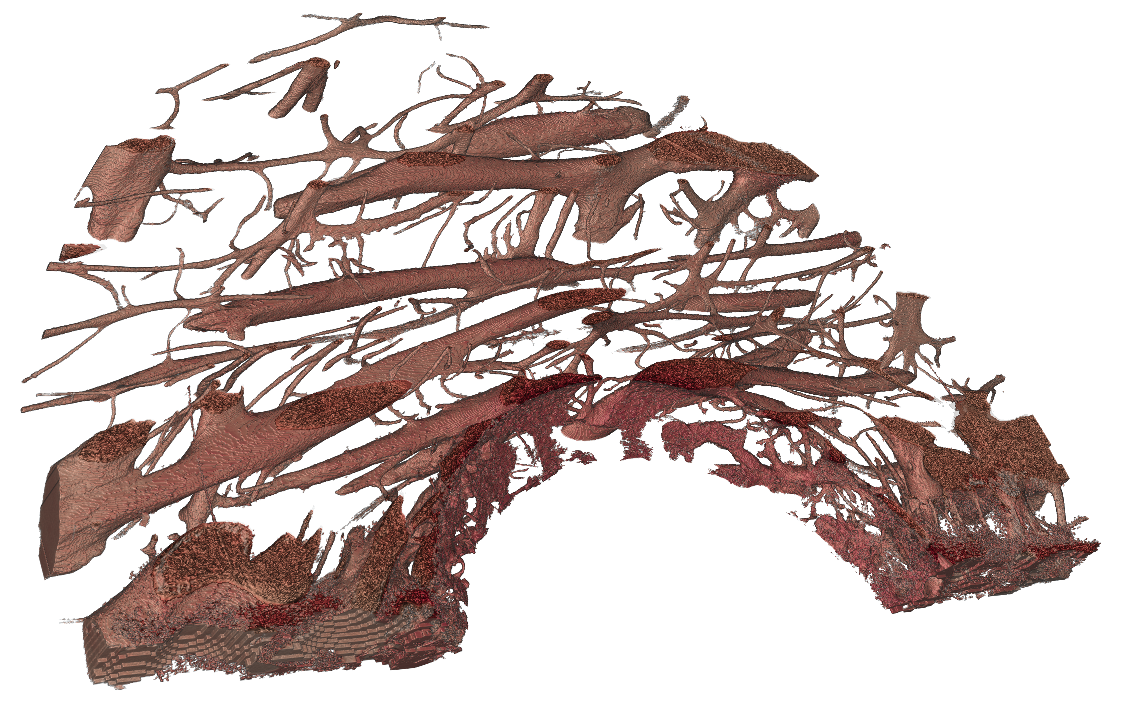
\includegraphics[width=\linewidth]{figures/blood_old_bone_100.png}
        % TODO opdater hvis en anden slice størrelse bliver brugt. voxel size = 3.75
        \caption{3D render of a $375\mu m \times 4230\mu m \times 6480\mu m$ slice of the blood network in the old bone region.}
        \label{fig:blood-old-slice}
    \end{subfigure}
    \begin{subfigure}[b]{\linewidth}
        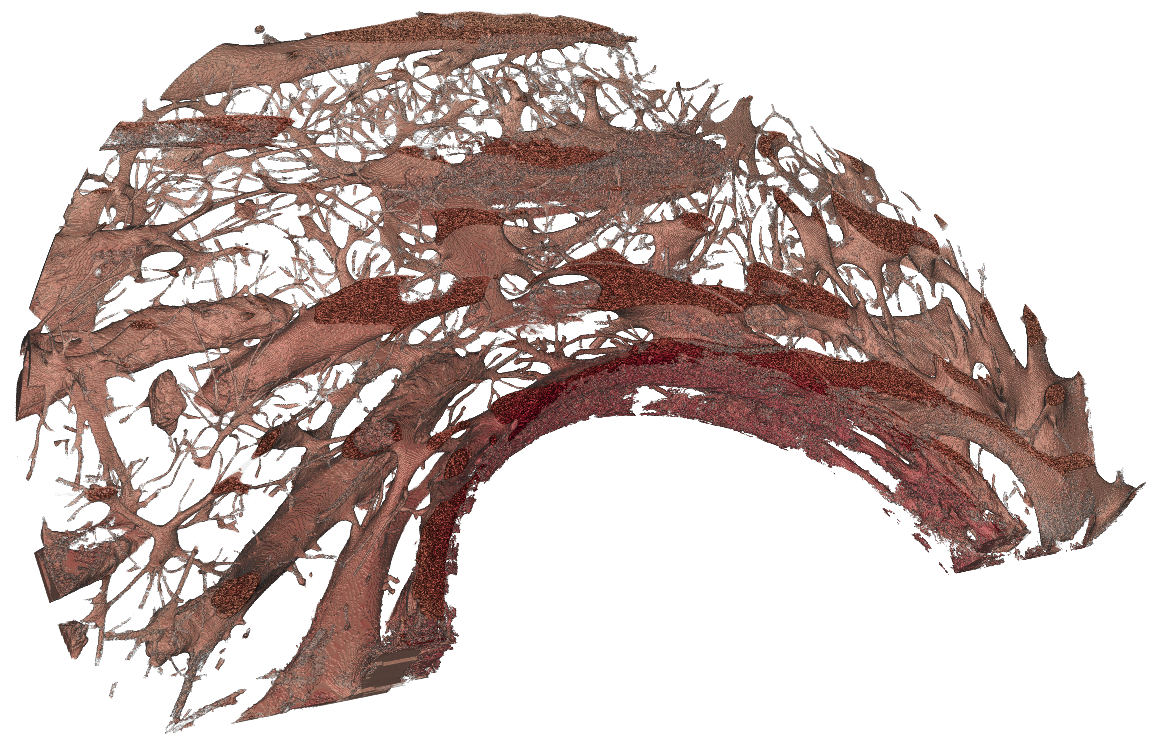
\includegraphics[width=\linewidth]{figures/blood_new_bone_100.png}
        \caption{3D render of a $375\mu m \times 4230\mu m \times 6480\mu m$ slice of the blood network in the new bone region.}
        \label{fig:blood-new-slice}
    \end{subfigure}
    \begin{subfigure}[b]{.45\linewidth}
        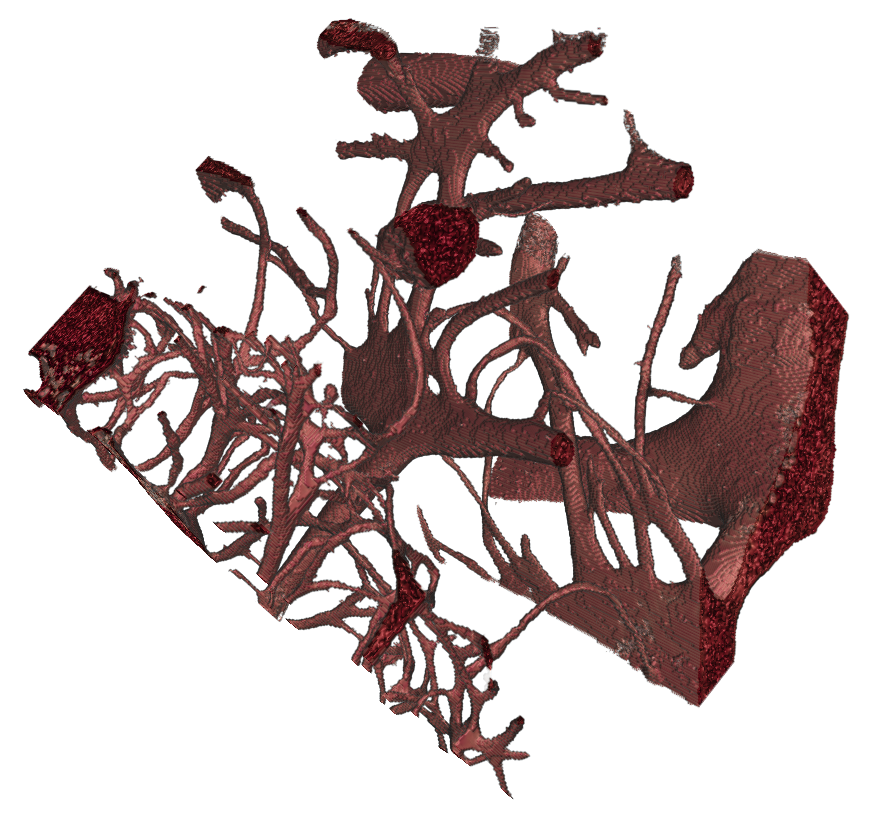
\includegraphics[width=\linewidth,height=\linewidth]{figures/blood_old_cube.png}
        \caption{3D render of a $1mm \times 1 mm \times 1 mm$ cube of the blood network in the old bone region.}
        \label{fig:blood-old-cube}
    \end{subfigure}
    \hfill
    \begin{subfigure}[b]{.45\linewidth}
        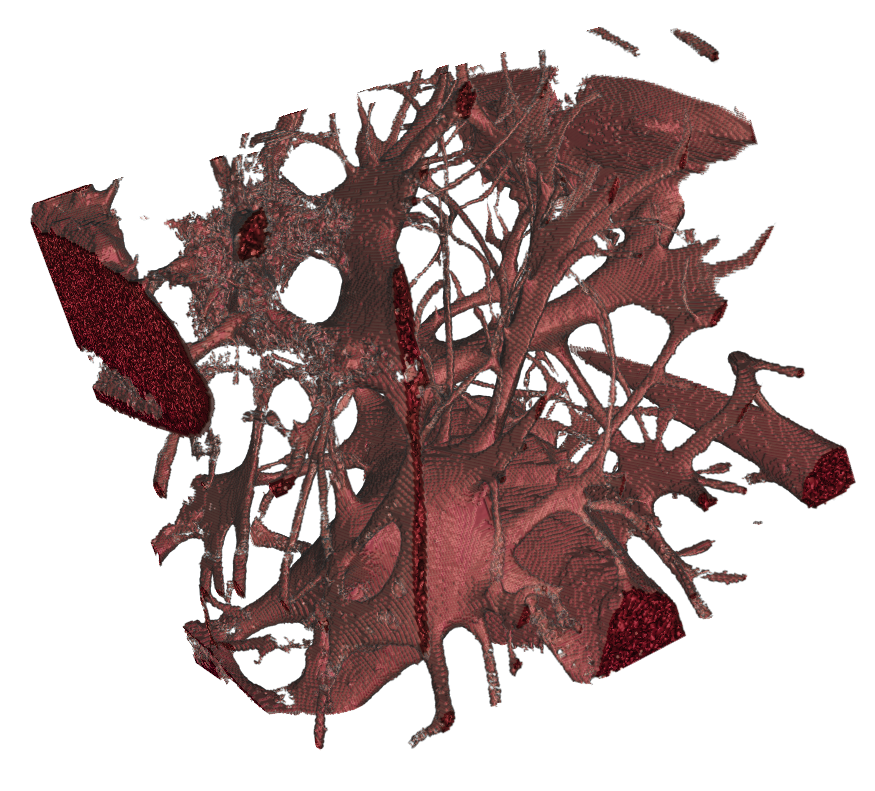
\includegraphics[width=\linewidth,height=\linewidth]{figures/blood_new_cube.png}
        \caption{3D render of a $1mm \times 1 mm \times 1 mm$ cube of the blood network in the new bone region.}
        \label{fig:blood-new-cube}
    \end{subfigure}
    \caption{3D renders of the blood network. All of the samples are generated from a 2x downsample of the full resolution. Note the difference between the the capillary network in the old bone region (\ref{fig:blood-old-slice},\ref{fig:blood-old-cube}) compared to the newly grown bone region (\ref{fig:blood-new-slice},\ref{fig:blood-new-cube}).}
    \label{fig:blood-network}
\end{figure}

\subsubsection{Sub-classification of soft tissue}

With a good separation of soft tissue and bone, we  map out the blood vessel network using connected
components analysis. The osteocytes are selected by volume and shape: For every connected component
in the feasible volume range, its principal axis and best ellipsoid is computed and checked against
the potential osteocyte shape.

\subsection{Visualizing bone-implant contact and blood-implant contact}

Once segmenter, tissue in contact with the implant can be studied using the
Euclidean Distance Transform (EDT) from the implant, restricted to the bone region. We can
simply mask the voxels that are within a thin shell of distances, $d_{min} < d(x,y,z) \le d_{max}$,
for example $d_{min} = 1\mu m$ to $d_{max} = 10\mu m$. We then sum over the masked voxels of each
tissue type to obtain and divide by the total to obtain the tissue-to-implant contact per area,
or study the distribution across the surface area qualitatively.

\subsubsection{Histology-comparison}

\begin{figure}
  \centering
  \begin{tabular}{c}
    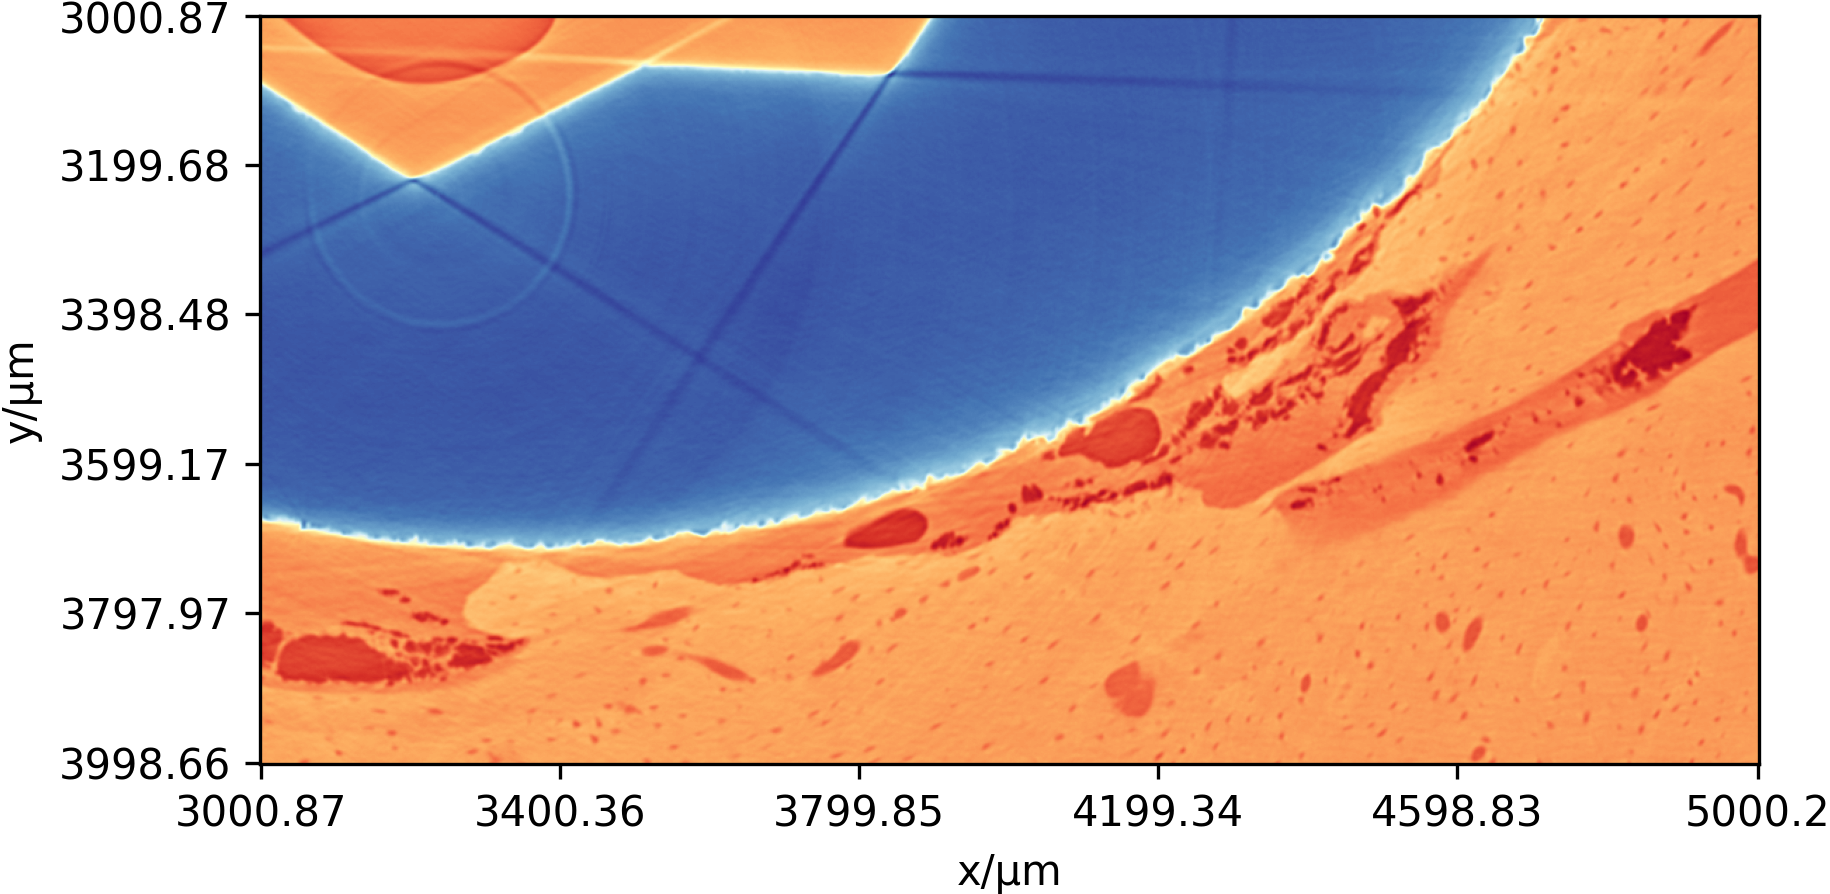
\includegraphics[width=\linewidth]{770c_pag-bic-xy-1x} \\
    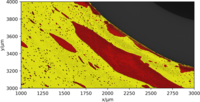
\includegraphics[width=\linewidth]{770c_pag-bic-P01-xy-1x}
  \end{tabular}
  \caption{TBW}
  \label{fig:histology-comparison1}
\end{figure}

\begin{figure}
  \centering
  \begin{tabular}{c}
    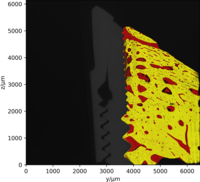
\includegraphics[width=\linewidth]{770c_pag-full-P01-yz-1x} \\
    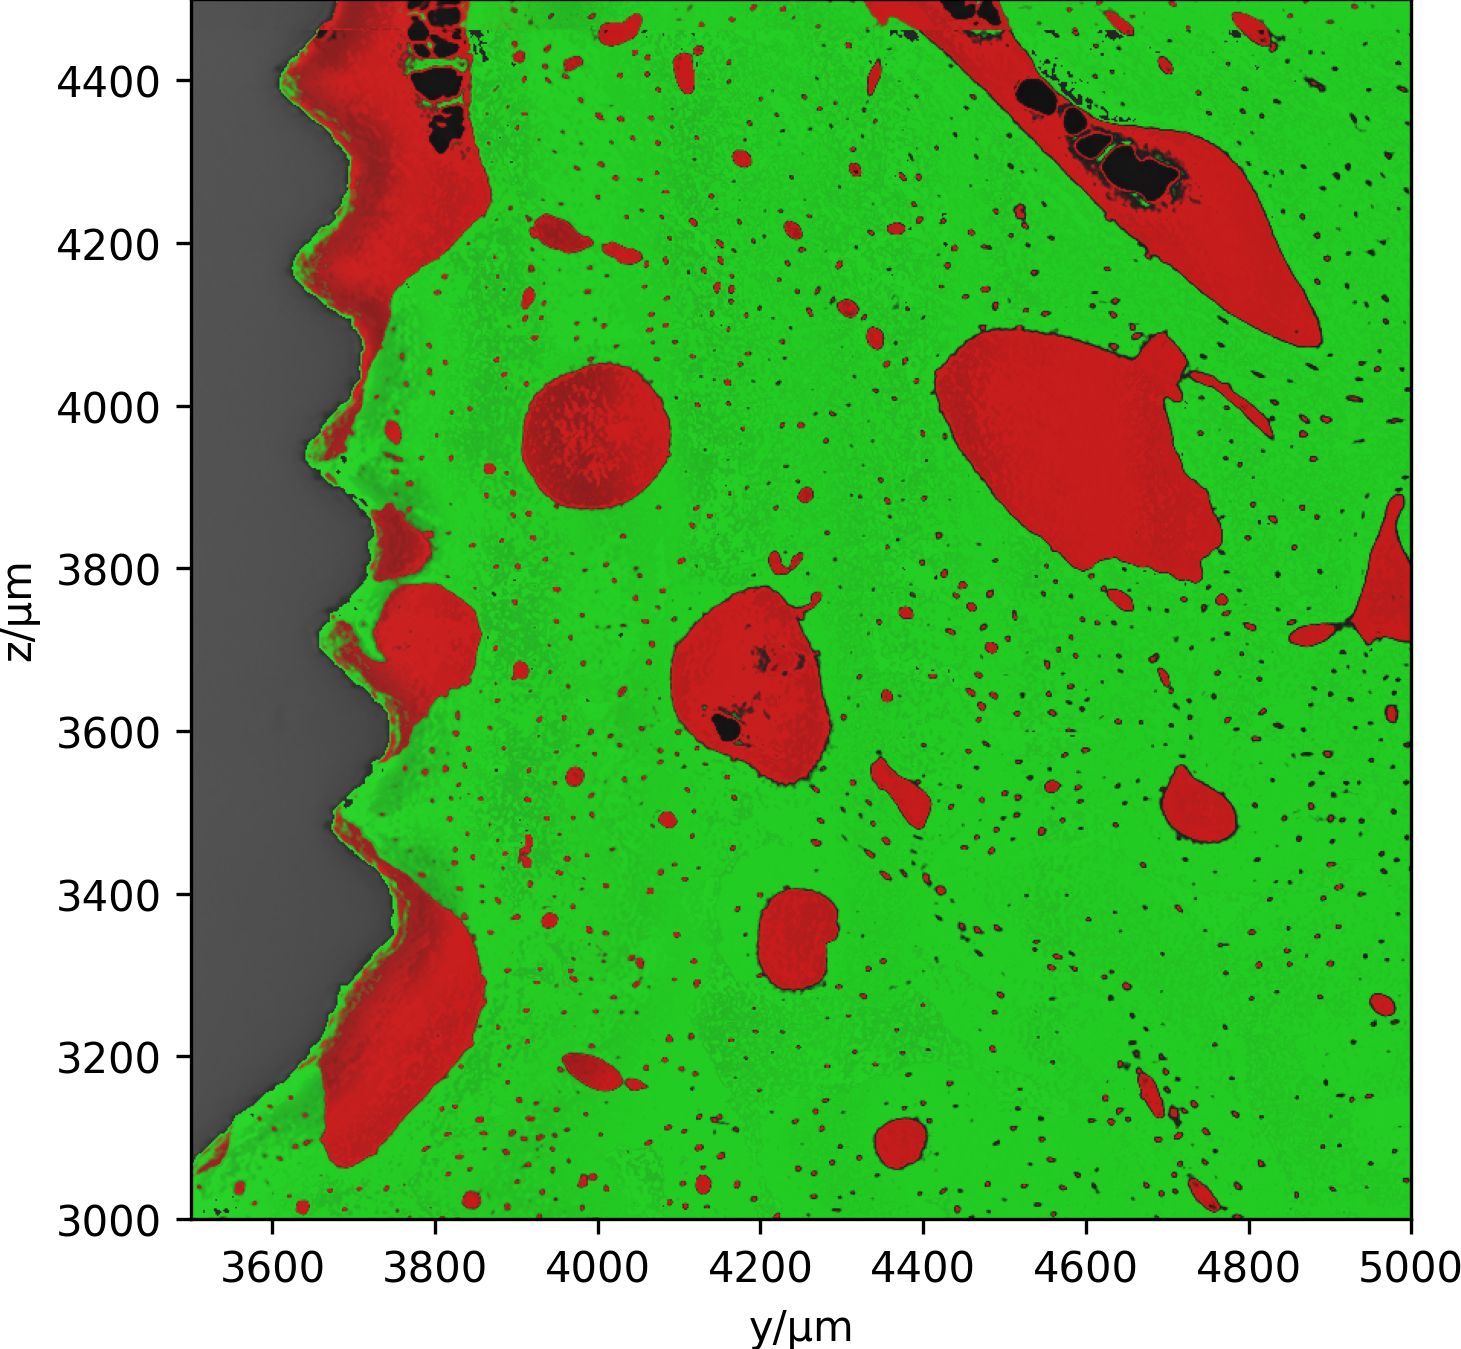
\includegraphics[width=\linewidth]{770c_pag-bic-P01-yz-1x}
  \end{tabular}
  \caption{TBW}
  \label{fig:histology-comparison2}
\end{figure}

% \subsubsection{Cylindrical projection of implant contact-surface}

% In this subsection, we show how to map the tissue-to-implant contact surface for visual inspection.
% The challenge is that the equidistant region forms a curved surface that cannot simply be flattened.
% Instead, we project the voxels onto a cylinder, as shown in Figure \ref{fig:cylinder1}.

% \begin{figure}
%   \centering
%   \begin{tabular}{cc}
%     (a) & \begin{tabular}{c}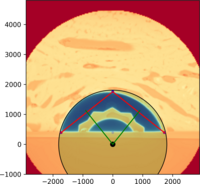
\includegraphics[width=.8\linewidth]{implant-FoR_prime-circle}\end{tabular} \\
%     (b) & \begin{tabular}{c}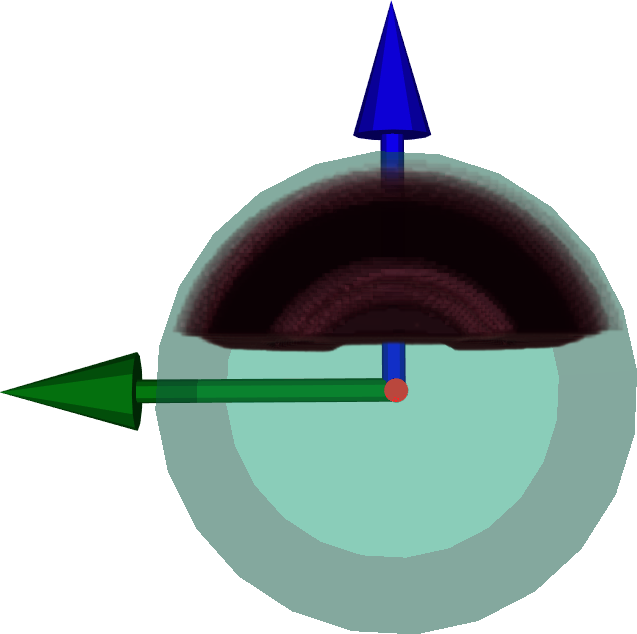
\includegraphics[width=0.4\linewidth]{implant-FoR_cylinder-y}%
%   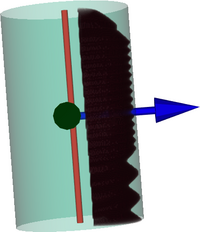
\includegraphics[width=0.5\linewidth]{implant-FoR_cylinder-z2}\end{tabular}
%   \end{tabular}
%   \caption{
%     (a) The implant is divided into 100 segments along its principal axis,
%     and for each segment, the circumscribed circle is computed.
%     (b) The best overall cylindrical fit for the implant is computed using
%     least squares. The implant contact is projected onto this cylinder,
%     and can now be shown in a flat plot.}
%   \label{fig:cylinder1}
% \end{figure}





%%% Local Variables:
%%% mode: latex
%%% TeX-master: "main"
%%% End:


%% main text
\section{Note}
\label{sec1}
Please use \verb+elsarticle.cls+ for typesetting your paper.
Additionally load the package \verb+medima.sty+ in the preamble using
the following command: 
\begin{verbatim} 
  \usepackage{medima}
\end{verbatim}

Following commands are defined for this journal which are not in
\verb+elsarticle.cls+. 
\begin{verbatim}
  \received{}
  \finalform{}
  \accepted{}
  \availableonline{}
  \communicated{}
\end{verbatim}

Any instructions relavant to the \verb+elsarticle.cls+ are applicable
here as well. See the online instruction available on:
\makeatletter
\if@twocolumn
\begin{verbatim}
 http://support.stmdocs.com/wiki/
 index.php?title=Elsarticle.cls
\end{verbatim}
\else
\begin{verbatim}
 http://support.stmdocs.com/wiki/index.php?title=Elsarticle.cls
\end{verbatim}
\fi

\subsection{Entering text}
\textcolor{newcolor}{\bf There is no page limit.}

\section{The first page}
Avoid using abbreviations in the title. Next, list all authors with
their first names or initials and surnames (in that order). Indicate
the author for correspondence (see elsarticle documentation).

Present addresses can be inserted as footnotes. After having listed all
authors' names, you should list their respective affiliations. Link
authors and affiliations using superscript lower case letters.

\subsection{The Abstract}
An Abstract is required for every paper; it should succinctly summarize
the reason for the work, the main findings, and the conclusions of the
study. The abstract should be no longer than 200 words. Do not include
artwork, tables, elaborate equations or references to other parts of
the paper or to the reference listing at the end. ``Comment'' papers
are exceptions, where the commented paper should be referenced in full
in the Abstract.

The reason is that the Abstract should be understandable in itself to
be suitable for storage in textual information retrieval systems.

\textit{Example of an abstract: A biometric sample collected in an
uncontrolled outdoor environment varies significantly from its
indoor version. Sample variations due to outdoor environmental
conditions degrade the performance of biometric systems that
otherwise perform well with indoor samples. In this study, we
quantitatively evaluate such performance degradation in the case
of a face and a voice biometric system. We also investigate how
elementary combination schemes involving min-max or z
normalization followed by the sum or max fusion rule can
improve performance of the multi-biometric system. We use
commercial biometric systems to collect face and voice samples
from the same subjects in an environment that closely mimics the
operational scenario. This realistic evaluation on a dataset of
116 subjects shows that the system performance degrades in
outdoor scenarios but by multimodal score fusion the
performance is enhanced by 20\%. We also find that max rule
fusion performs better than sum rule fusion on this dataset. More
interestingly, we see that by using multiple samples of the same
biometric modality, the performance of a unimodal system can
approach that of a multimodal system.}

\section{The main text}

Please divide your article into (numbered) sections (You can find the
information about the sections at
\url{http://www.elsevier.com/wps/find/journaldescription.cws_home/505619/authorinstructions}).
Ensure that all tables, figures and schemes are cited in the text in
numerical order. Trade names should have an initial capital letter, and
trademark protection should be acknowledged in the standard fashion,
using the superscripted characters for trademarks and registered
trademarks respectively. All measurements and data should be given in
SI units where possible, or other internationally accepted units.
Abbreviations should be used consistently throughout the text, and all
nonstandard abbreviations should be defined on first usage
[removed].

\begin{table*}[!t]
\caption{\label{tab1}Summary of different works pertaining to face and
speech fusion}
\centering
\begin{tabular}{|p{2.25cm}|p{2cm}|l|p{4cm}|p{3cm}|p{2cm}|}
\hline
Study & Algorithm used & DB Size & Covariates of interest & 
Top individual performance & Fusion\newline Performance\\
\hline
UK-BWG
(Mansfield et al.,
2001) &
Face, voice:\newline
Commercial & 200 & Time: 1--2 month\newline
separation (indoor) & 
TAR$^*$ at 1\% FAR$^{\#}$\newline
Face: 96.5\%\newline
Voice: 96\%
& --\\
\hline
Brunelli
(Brunelli and
Falavigna, 1995) & 
Face:\newline
Hierarchical\newline
correlation\newline
Voice:\newline
MFCC & 
87 & 
Time: 3 sessions, time\newline
unknown (indoor) & 
Face:\newline
TAR = 92\% at\newline
4.5\% FAR\newline
Voice:\newline
TAR = 63\% at\newline
15\% FAR
&
TAR =98.5\%\newline
at 0.5\% FAR\\
\hline
Jain
(Jain et al., 1999)
&
Face:\newline
Eigenface\newline
Voice:\newline
Cepstrum\newline
Coeff. Based
&
50
&
Time: Two weeks (indoor)
&
TAR at 1\% FAR\newline
Face: 43\%\newline
Voice: 96.5\%\newline
Fingerprint: 96\%
& 
Face $+$ Voice $+$\newline
Fingerprint $=$\newline
98.5\%\\
\hline
Sanderson
(Sanderson and
Paliwal, 2002)
&
Face: PCA\newline
Voice: MFCC &
43 
& Time: 3 sessions (indoor)\newline
Noise addition to voice & 
Equal Error Rate\newline
Face: 10\%\newline
Voice: 12.41\%
&
Equal Error\newline
Rate 2.86\% \\
\hline
Proposed study & 
Face, voice:\newline
Commercial & 116 &
Location: Indoor and\newline
Outdoor (same day)\newline
Noise addition to eye\newline 
coordinates 
&
TARs at 1\% FAR\newline
Indoor-Outdoor\newline
Face: 80\%\newline
Voice: 67.5\%
&
TAR = 98\%\newline
at 1\% FAR\\
\hline
\multicolumn{6}{@{}l}{$^*$TAR--True Acceptance Rate\qquad 
$^{\#}$ FAR--False Acceptance Rate}
\end{tabular}
\end{table*}


\subsection{Tables, figures and schemes}
Graphics and tables may be positioned as they should appear in the
final manuscript. Figures, Schemes, and Tables should be numbered.
Structures in schemes should also be numbered consecutively, for ease
of discussion and reference in the text. \textcolor{newcolor}{\bf
Figures should be maximum half a page size.}

Depending on the
amount of detail, you can choose to display artwork in one column (20
pica wide) or across the page (42 pica wide). Scale your artwork in
your graphics program before incorporating it in your text. If the
artwork turns out to be too large or too small, resize it again in your
graphics program and re-import it. The text should not run along the
sides of any figure. This is an example for citation [removed].

\begin{figure}[!t]
\centering
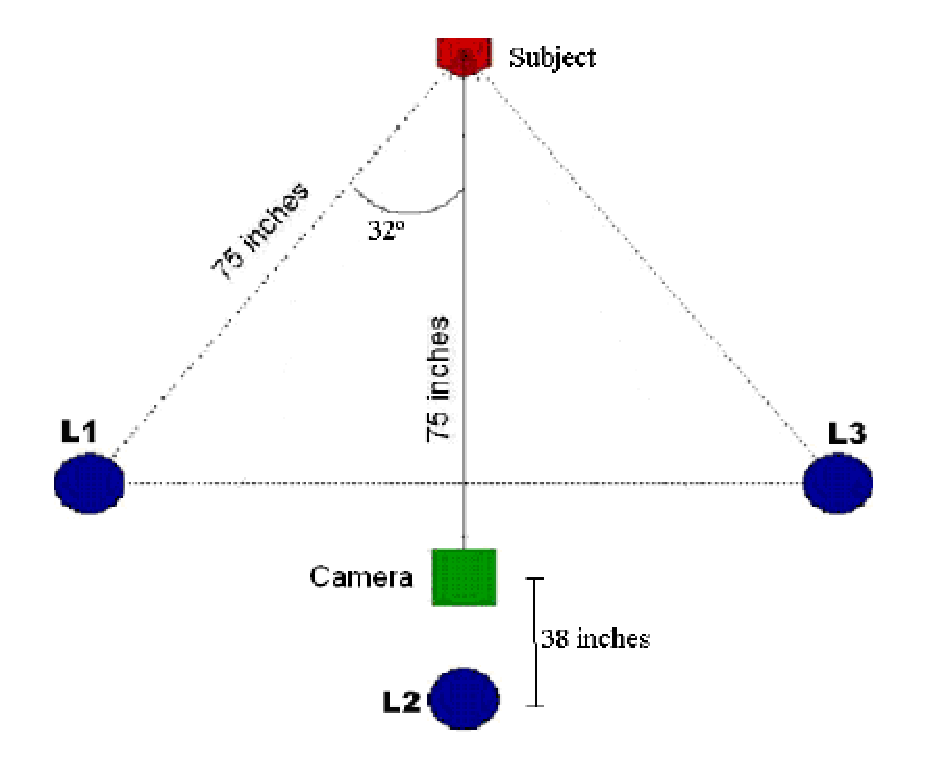
\includegraphics[scale=.5]{medimafig01}
\caption{Studio setup for capturing face images indoor. Three light
sources L1, L2, L3 were used in conjunction with normal office lights.}
\end{figure}

You might find positioning your artwork within the text difficult
anyway. In that case you may choose to place all artwork at the end of
the text and insert a marker in the text at the desired place. In any
case, please keep in mind that the placement of artwork may vary
somewhat in relation to the page lay-out [removed].

This can easily be achieved using \verb+endfloat.sty+ package. Please
refer the following documentation to use this package.
\makeatletter
\if@twocolumn
\begin{verbatim}
  http://mirrors.ctan.org/macros/latex/contrib/
  endfloat/endfloat.pdf
\end{verbatim}
\else
\begin{verbatim}
  http://mirrors.ctan.org/macros/latex/contrib/endfloat/endfloat.pdf
\end{verbatim}
\fi
\makeatother

\textcolor{newcolor}{\bf You should insert a caption for the figures
below the figures and for the tables the caption should be above the
tables.} 

Please remember that we will always also need highresolution versions
of your artwork for printing, submitted as separate files in standard
format (i.e. TIFF or EPS), not included in the text document. Before
preparing your artwork, please take a look at our Web page:
\url{http://www.elsevier.com/locate/authorartwork}.


\subsection{Lists}

For tabular summations that do not deserve to be presented as
a table, lists are often used. Lists may be either numbered or
bulleted. Below you see examples of both.
\begin{enumerate}
\item The first entry in this list
\item The second entry
\begin{enumerate}
\item A subentry
\end{enumerate}
\item The last entry
\end{enumerate}
\begin{itemize}
\item A bulleted list item
\item Another one
\end{itemize}

\subsection{Equations}
Conventionally, in mathematical equations, variables and
anything that represents a value appear in italics.
All equations should be numbered for easy referencing. The number
should appear at the right margin.
\begin{equation}
S_{\rm pg}'=\frac{S_{\rm pg}-\min(S_{\rm pG})}
 {\max(S_{\rm pG}-\min(S_{\rm pG})}
\end{equation}
In mathematical expressions in running text ``/'' should be used for
division (not a horizontal line). 

\section*{Acknowledgments}
Acknowledgments should be inserted at the end of the paper, before the
references, not as a footnote to the title. Use the unnumbered
Acknowledgements Head style for the Acknowledgments heading.

\section*{References}

Please ensure that every reference cited in the text is also present in
the reference list (and vice versa).

\section*{\itshape Reference style}

Text: All citations in the text should refer to:
\begin{enumerate}
\item Single author: the author's name (without initials, unless there
is ambiguity) and the year of publication;
\item Two authors: both authors' names and the year of publication;
\item Three or more authors: first author's name followed by `et al.'
and the year of publication.
\end{enumerate}
Citations may be made directly (or parenthetically). Groups of
references should be listed first alphabetically, then chronologically.


\section*{Supplementary Material}

Supplementary material that may be helpful in the review process should
be prepared and provided as a separate electronic file. That file can
then be transformed into PDF format and submitted along with the
manuscript and graphic files to the appropriate editorial office.



\bibliographystyle{model2-names.bst}\biboptions{authoryear}
\bibliography{refs}
\end{document}